% v3, 4 November 2026. Author metadata is intentionally absent in this review copy.
\documentclass[pre,twocolumn,superscriptaddress,showpacs,floatfix]{revtex4-2}
\usepackage{amsmath,amssymb,bm,graphicx,xcolor}
\usepackage{xr-hyper}
\usepackage[colorlinks=true,linkcolor=blue!60!black,citecolor=blue!60!black,urlcolor=blue!60!black]{hyperref}
\newcommand{\qs}{q^{*}}
\newcommand{\ds}{\mathrm{d}}

\externaldocument[M-]{main}
\renewcommand{\thesection}{S\Roman{section}}
\renewcommand{\thefigure}{S\arabic{figure}}
\renewcommand{\thetable}{S\Roman{table}}
\renewcommand{\theequation}{S\arabic{equation}}
\begin{document}
\title{Supplemental material: Discontinuous transition into two symmetric absorbing states in two dimensions}
\date{4 November 2026}
\maketitle
\raggedbottom
\setlength{\parskip}{0pt}
This supplement supplies the detailed windows, geometries, finite-size
comparisons and model checks for the accompanying paper.
Labels without an S prefix refer to the main paper. Numerical intervals
retain their stated sampling assumptions; reference, estimator and observation
window sensitivity are reported separately.

\section{Simulation protocols and statistical conventions}
\label{sec:protocols}

\textit{Simulation.} We use a bit-parallel implementation in which each 64-bit word holds 64
sites and the neighbor counts and flip decisions are computed with bitwise operations. Each site
draws one uniform random number per step and flips if it is below the flip probability of its
class $(\sigma_i, j_i)$; all classes of a word share one bit-serial comparison, so the cost does
not depend on the number of distinct flip probabilities. Random numbers come from the
counter-based Philox$4\times 32$-10 generator~\cite{salmon2011}, keyed by the run's seed and
indexed by (time, row, word), so every run is bit-for-bit reproducible independently of the
number of threads and of restarts from checkpoints. The code passes a bit-exact comparison with a
naive per-site implementation for several rules and lattice shapes, and statistical tests of
the per-class flip frequencies (Supplemental Sec.~\ref{app:numerics}). Near the transition it performs
about $10^9$ site updates per second per core. The extended dense-lattice
campaign uses a CUDA backend built from the same integer update and random-number
functions. CPU and GPU outputs agree bit for bit in the validation cases,
including large lattices, directed profiles, and checkpoints transferred in
both directions (Supplemental Sec.~\ref{app:numerics}).

\textit{Protocols.} We use five kinds of runs.
(i) \emph{Bulk}: random initial condition with density $1/2$ on an $L\times L$ torus.
(ii) \emph{Strip fronts}: on an $L_x\times L_y$ torus, the rows $y<L_y/2$ start random and the
rest dead, giving two flat fronts between the active phase and the absorbing state. The per-row
interface counts are recorded, each front is located at a fixed fraction of
the relaxed interior activity, and the velocity $v$ is half the slope of the
strip width, $W(t) = W_0 + 2vt$,
fitted while the geometry remains a separated pair of fronts. The reference
level and validity windows are specified in Sec.~\ref{app:numerics}.
(iii) \emph{Tilted bands}: a band of direction $(a,b)$, the sites with
$(a y - b x)\bmod L < L/2$, on an $L\times L$ torus. Its two edges have total length
$2L\sqrt{a^2+b^2}$. Profiles binned along the normal locate both edges directly;
their separation gives the normal velocity without converting total activity
into an area.
(iv) \emph{Droplets and seeds}: a disk of radius $R$ whose sites are alive with probability $1/2$
(or a $2\times 2$ block of live sites) in the all-dead state. Many independent replicas are run;
since a site with $j = 0$ never flips, only the bounding box of the active region needs to be
updated, which is exact and makes each replica cheap. A replica stops when it
dies, reaches the lattice edge, or reaches its declared time horizon.
For the droplet experiment, $P_{\rm grow}$ is the probability of reaching
the edge before extinction and before that horizon. In seed-survival curves,
escaped replicas are retained as a separately recorded contribution; they
bound rather than directly measure survival after escape.
(v) \emph{Walls}: all-alive rows $y<L_y/2$ and all-dead rows above, i.e., two flat walls between
the two absorbing phases and no active phase at $t = 0$.
Times are in steps (one synchronous update of all sites). Error bars are standard errors over
independent runs unless stated otherwise.

\textit{Statistical analysis.} The reanalyzed flagship bulk data and the new
fixed-manifest campaigns use every run in complete, predetermined seed groups,
with no density filter or conditioning on survival. Supporting parameter surveys
retain their separately stated windows and selection protocols.
A partially finished fixed group is retained for diagnostics but not
used as an unconditional ensemble: absorption can make a run finish sooner
than a surviving trajectory. We integrate each sampled
trajectory in time before averaging independent runs; a trajectory is extended
by its known constant state after absorption. The half-density time is the first
recorded crossing of $\rho<0.145$ after $t=10^3$, half a reference density
$\rho_{\rm ref}=0.29$ near the flagship transition. It is distinct from complete
consensus. Five legacy $L=64$ runs already below this threshold at the analysis
origin are marked left censored at $10^3$, with lower bound zero. Other
first observed crossings retain the preceding output time as a recording-grid
diagnostic. Activity is not monotone, so brief unobserved dips can occur earlier;
these brackets are not rigorous bounds on its first physical passage.
Unobserved events are right censored, and survival curves and restricted mean times retain
that censoring. An event-free ensemble supplies right-censored observations
and a bound on finite-time survival, not a measured mean lifetime.
Independent-run resampling gives the reported bootstrap
intervals. For the four-run large-system groups these are approximate measures
of observed run variation and do not account for rare outcomes absent from
the sample. Event counts and systematic fitting-window checks are reported
separately.

%=====================================================================================

The percentile intervals for four-run ensembles are displayed as conditional
summaries of observed run variation, not calibrated $95\%$ error guarantees.
We show individual paired changes where their sign is used in the text.
For the two small directional contrasts and midpoint density drift we also
report a small-sample $t$ reference calculation, keeping its normality and
linearization assumptions explicit. Neither method substitutes for more
independent trajectories when precise tail coverage is essential.

\section{Numerical details}
\label{app:numerics}

For complete simulation protocols, see Sec.~\ref{sec:protocols}.

\textit{Code.} The simulator stores 64 sites per 64-bit word. The eight neighbor bits of all sites
of a word are summed with bitwise adder trees, giving the number of live neighbors $k$ in four
bit planes; the flip class of each site is $(\sigma, k)$, with the flip probability $f_{\sigma k}$
read from an $2\times 9$ table, so that any outer-totalistic rule, Eq.~\eqref{M-eq:rule}, and the lazy
tables of Sec.~\ref{sec:async} are run by the same kernel. Each site draws one 32-bit uniform per
step from Philox$4\times32$-10~\cite{salmon2011} with counter (time, row, word, draw), and the 64
comparisons with the per-class thresholds are done bit-serially in parallel. Validation: (i) a
bit-exact comparison with a naive per-site implementation for five rules on four lattice shapes,
including one-word-wide and three-row lattices; (ii) per-class flip frequencies for an 18-class
table (variance of the $z$ scores over 560 repetitions $1.04\pm0.06$) and a $1.3\times10^8$-sample
test of the shared comparison on a voter-like table (per-class frequencies and adjacent-lane
independence, $|z|<2$); (iii) identical output for any number of threads and across restarts
from checkpoints; (iv) agreement with an independent GPU implementation of the $p = 0$ model to
1\% in the stationary density.

\textit{CUDA extension.} The dense GPU backend uses the original CPU integer
flip function and Philox implementation, extracted automatically into device
code. Two lattice buffers implement simultaneous updates; batches of 256 steps
are submitted as CUDA graphs without changing the update order or counters.
The host retains initialization, observables, profiles, and checkpoint format.
Validation compares full configurations, time series, profiles, snapshots, and
checkpoints byte for byte with the CPU implementation. Cases include one-word
rows, an $L=2048$ lattice, Moore and von Neumann neighborhoods, lazy update
tables, irregular output schedules, graph-batch boundaries, and counters near
$2^{32}$. CPU-to-GPU and GPU-to-CPU restarts reproduce the same trajectories.
The GPU checks absorption at scheduled outputs, so its absorption times are
interval observed. The lifetime and sparse-replica campaigns use the CPU code.
Parameter manifests record distinct 64-bit seeds, source and executable hashes,
and completion status; interrupted runs are identified rather than silently
pooled with completed ensembles.

\textit{Replica mode.} For seeds and droplets, only the bounding box of the sites with a
disagreeing neighbor (plus a margin) is updated, refitted every 32 steps. This is exact because a
site with $j = 0$ cannot flip and its random numbers are indexed by position, not by the order
of updates; over 200 seeds, box and full-lattice updating give identical configurations at
every step. A replica whose box comes within 2 rows or 64 columns of the lattice edge is stopped
and recorded as an escape. Its later survival is unobserved; the
seed-curve convention retains it as a separately tabulated contribution,
while the droplet growth observable counts the escape itself. In the pure voter model the method reproduces the martingale
$\langle A(t)\rangle = 4$ for the number of live sites of a $2\times2$ seed (within $|z|<0.94$
at all 38 output times over $2\times10^5$ replicas) and $P_s(t)\propto\ln t/t$.

\textit{Front tracking.} The broad strip survey in Table~\ref{tab:line}
uses a smoothed row profile and local interpolation of the velocities bracketing
reversal. For the orientation, extended-strip, and $p=1/2$ lazy-update
analyses, we explicitly track
the outer envelope: the lowest and highest bins whose smoothed activity exceeds
$0.3$ of the interior reference value measured at $t=10^3$. An interior hole
cannot stop this envelope. We also retain the center-connected-component width,
interior activity, and hole fraction as diagnostics. No run is removed simply
because its interior density is small in these corrected analyses.
The other supporting parameter surveys retain their legacy center-connected
tracker and interior-activity validity criterion; their crossing estimates
are not assigned the precision of the extended campaign.

For a tilted band, $s=(ay-bx)\bmod L$ has $L$ bins containing $L$ sites each,
with normal spacing $1/\sqrt{a^2+b^2}$. Smoothing is over nine normal lattice
spacings, converted to an odd number of bins. The front speed is half the slope
of the normal width. Fits stop when the band leaves the width range
$[0.15L,0.85L]$ in bin coordinates, before winding or disappearance invalidates
the geometry. In the broad orientation survey the principal window begins at
$t=2\times10^4$; fits starting at $10^4$ and $4\times10^4$ and threshold
fractions 0.2, 0.3, and 0.5 quantify sensitivity. Local bracketing estimates,
linear fits over wider intervals, and quadratic fits are compared explicitly.
Independent runs are resampled within each $q$ for the crossing intervals;
uncertainty from the fit model or time window is reported separately. The
extended campaign additionally compares late and nonoverlapping time windows;
each published fit requires full coverage of its declared window for every seed.

\textit{Sampling uncertainty.} Independent realizations are the statistical
units; lattice sites and successive output records are not treated as
independent samples. For some scalar means and paired mean differences in the
four-run ensembles, the reductions enumerate all $4^4=256$ ordered
empirical bootstrap resamples; other retained reductions use Monte Carlo
resampling with the count recorded in their provenance. Enumeration removes Monte Carlo error in the
resampling calculation, not the limited coverage accuracy from four runs.
Front-crossing intervals additionally condition on the stated interpolation,
window, and geometrical eligibility. Pointwise intervals are distinguished
from the simultaneous orientation contrasts. Exact binomial intervals are
used for fixed-count survival endpoints. All these sampling intervals remain
separate from finite-size, finite-time, and estimator sensitivity.

\textit{Spatial correlations.} The large-system correlations are evaluated
directly from the final packed-bit configurations, using periodic shifts in
each coordinate direction. Each stored configuration is checked against its
recorded size, time, digest, magnetization, and nearest-neighbor activity;
the identity $C(1)=1-2\rho$ supplies an additional consistency check.
All declared runs are retained. The same resampled run indices are used at
every separation when constructing the pointwise uncertainty bands.
These final-time measurements do not assume an exponential correlation form.

\textit{Droplets and holes.} For a row with live count $n_y$, the signed chord is $c_y=2n_y$ for an
active disk and $c_y=L-2n_y$ for an absorbing hole. The primary estimator is
$A=\sum_{|y-L/2|<1.3R_0+50}\max(c_y,0)$ with $R_0=1000$, followed by
$R=\sqrt{A/\pi}$. The crop reduces noise from the surrounding active phase;
rectification can introduce a positive area bias. We therefore also compute
$A_{\rm full}=\sum_y c_y$ and the trimmed signed sum, and report the resulting
rate sensitivity. Every such area stays positive in the retained trajectories.
Radius slopes are fitted over $2\times10^4\le t\le2\times10^5$.
The curvature overlays integrate the radius-dependent equation throughout
this window, with their initial radius fixed by the observed mean.


\textit{Layer edges.} For the roughness of the wetting layer (Sec.~\ref{sec:swall}) full
configurations were stored every $10^5$ steps. In each column the two edges of the layer are its
lowest and highest interface sites within $L_y/4$ of the wall; their variances along the wall and
the height-difference correlation $\langle[h(x+r)-h(x)]^2\rangle$ give the roughness.
These are two physical edges in the wall geometry. The same two-extrema
rule applied to a half-active band mixes its exterior front with an artificial
window boundary inside the active bulk. We therefore omit the previous
free-band comparator. The original band snapshots needed to replace that
curve are absent from the local data release; no corrected numerical
comparison is inferred from other snapshots.

\textit{Cost.} The earlier CPU campaigns used approximately 2200 core hours,
on Intel Xeon Platinum 8592+ nodes and a workstation, at
$(0.9$--$2.8)\times10^9$ site updates per second per core. The additional
campaign used 58.4 GPU allocation hours on NVIDIA H200 devices and
99.0 CPU-only allocated core hours. These allocation totals include validation,
I/O, and failed or restarted attempts; GPU-host CPU allocations are recorded
separately. Across the 40 staged GPU workers, mean sampled utilization during
simulation runs ranged from 92.7\% to 99.9\%. These samples include in-run
I/O but exclude build, validation, inter-task staging, and each run's initial
20 seconds; they are not allocation-wide efficiency estimates.

The additional front uncertainty check linearizes each locally interpolated
zero with respect to the two bracketing group means. It combines independent
within-group sample variances with Welch--Satterthwaite degrees of freedom.
For temporal contrasts, the same run's early and late linearized contributions
are paired before estimating variance. The angular contrast applies a
Bonferroni adjustment for the three pairwise direction comparisons. This is
a sensitivity calculation conditional on the observed bracket; it cannot
supply exact coverage from four runs or replace an assessment of systematic
front and finite-time effects.

\section{Front geometries, time windows, and large droplets}
\label{sec:sfronts}

A strip of the active phase next to the absorbing state grows on one side of
the transition and shrinks on the other. The broad survey places reversal
near $q=0.04592$; the longer measurements below refine this location.
Behind a retreating front, the interior retains a substantial interface-site
fraction ($\iota_{\rm in}\simeq0.71$ at $q\simeq0.0436$, compared with about
0.76 near reversal). The active region is therefore invaded coherently before
it disappears. At a continuous transition the asymptotic active density would
instead vanish at the boundary. A finite-time retreating interface alone
does not distinguish these cases; we compare it with bulk and nucleation
measurements below. Front reversal also locates phase competition in the
four-species alliance model~\cite{szabo2004} and in spatial bistable
systems~\cite{durrett1994,durrett2009}.

In nonequilibrium systems, the reversal point can depend on front orientation.
Between the extreme crossings, a window of generic coexistence can open in
which sufficiently large droplets of either phase shrink by
faceting~\cite{toom1980,bennett1985,wang2015}. We compare bands with normals
$(1,0)$, $(2,1)$, and $(1,1)$, at $0^\circ$, $26.6^\circ$, and $45^\circ$
to the axes. Figure~\ref{fig:orient} shows the broad survey at $p=0.1$, $1/2$,
and $0.9$, with $L=4096$, eight seeds per point, and $T=2\times10^5$.
The outermost threshold crossings of the smoothed profile locate the band;
interior holes do not terminate this envelope. The smoothing length is nine
lattice spacings in the physical normal direction for every orientation.

At $p=1/2$, local interpolation between the two points bracketing reversal,
using $t\ge2\times10^4$, gives $q^*=0.045919$, 0.045911, and 0.045923 for
these three normals. Their conditional 95\% seed-bootstrap intervals are
$[0.045912,0.045927]$, $[0.045902,0.045921]$, and
$[0.045912,0.045933]$, respectively. Time windows, threshold levels, and fit
curvature are varied separately to assess systematic sensitivity. Several
straight-line fits across the entire sampled range have significant lack of
fit; their formal errors are not used as the full uncertainty of a crossing.
The broad survey finds only small orientation differences, but does not by
itself establish a unique orientation-independent transition point. It
constrains a broad generic-coexistence window of the type observed in
Ref.~\cite{wang2015} and motivates the finer comparisons below.

\begin{figure*}
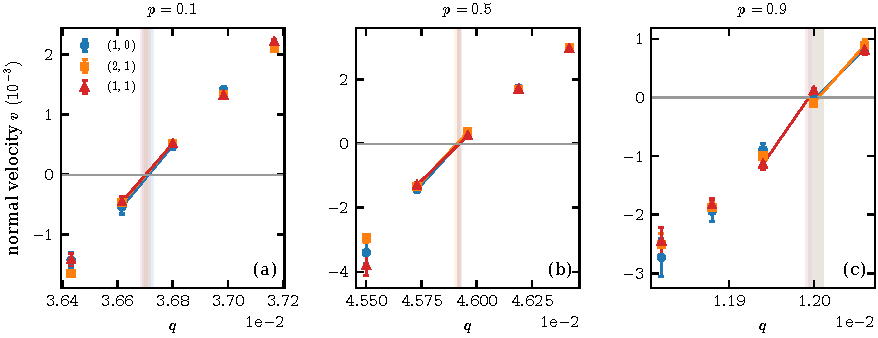
\includegraphics[width=\textwidth]{figs/fig_orient}
\caption{Normal velocity of a band of the active phase against the absorbing state, for normal
directions $(1,0)$, $(2,1)$, and $(1,1)$, at $p = 0.1$, $1/2$, and $0.9$; $L = 4096$, $T = 2\times10^5$,
eight seeds per point, velocity from the width of the band tracked along its normal for
$t\ge2\times10^4$. The horizontal coordinate is the actual probability $q$.
Lines interpolate the two seed-averaged velocities bracketing reversal;
shaded bands are conditional 95\% run-bootstrap intervals for the crossing.
Smoothing uses the same physical normal length for all orientations.
Farther below reversal the strip can nucleate absorbing domains internally,
so the broad-range velocity curve need not be linear.}
\label{fig:orient}
\end{figure*}

The fine-grid campaign extends these tests to $L=8192$ and 16384 and
$T=2\times10^6$ (Fig.~\ref{fig:gpu_fronts}). At $L=8192$, all five
probabilities and all three orientations have four completed independent
runs. Over $10^6\le t\le2\times10^6$, the local crossings are
0.0459387, 0.0459396, and 0.0459398 for normals $(1,0)$, $(2,1)$,
and $(1,1)$, respectively. Their spread is $1.0\times10^{-6}$, with a
conditional 95\% bootstrap upper value of $1.02\times10^{-5}$; simultaneous
pairwise intervals include zero. Varying the profile threshold from 0.2
to 0.5 gives crossings spanning 0.0459371--0.0459442 at this size and
window. At $L=16384$, the axial and tilted crossings differ by
$4.7\times10^{-6}$, with a simultaneous 95\% bootstrap interval
$[2.3,8.5]\times10^{-6}$. A small direction contrast is present in this finite geometry and window.
Its inferred precision depends on the estimator and uncertainty method,
as quantified below; it does not determine an asymptotic anisotropy.
The shift relative to the short survey also shows why
observation time must enter the uncertainty assessment.

\begin{figure*}
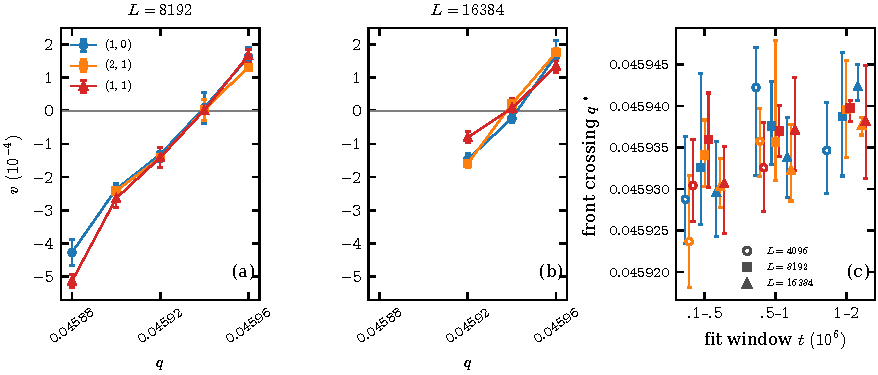
\includegraphics[width=\textwidth]{figs/fig_gpu_fronts}
\caption{Fine-grid front measurements at $p=\alpha=1/2$.
(a,b) Normal velocities at $L=8192$ and $16384$, fitted over
$10^6\le t\le2\times10^6$; four independent bands per point, and bars are
one standard error over runs. The profile threshold is 0.3 of the
reference activity at $t=10^3$. Colors and markers distinguish the three band
normals. Each included group retains a separated pair of fronts throughout
the stated fit window in every run.
(c) Local bracketing estimates of the velocity zero for three successive
windows; colors denote the same normals, while marker shapes denote $L$.
The $L=4096$ groups have eight runs, and the larger sizes four.
Intervals are conditional 95\% run-bootstrap intervals for each chosen
window and threshold. The variation between windows and orientations is
shown separately from sampling uncertainty.}
\label{fig:gpu_fronts}
\end{figure*}

Independent $L=8192$ cohorts followed to $5\times10^6$ steps test the
remaining time dependence (Fig.~\ref{fig:gpu_fronts5m}). For axial bands,
four new runs at each of $q=0.04593$, 0.04594, and 0.04595 give a crossing
of 0.0459340 over $2$--$3.5\times10^6$ and 0.0459435 over
$3.5$--$5\times10^6$. Resampling the same runs in the two windows gives
a paired shift of $9.4\times10^{-6}$ with a conditional 95\% interval
$[4.9,12.1]\times10^{-6}$. The change has the same sign at profile
thresholds 0.2 and 0.5. All fitted bands remain geometrically valid;
at $q=0.04594$, all four interiors retain more than 90\% of the reference
activity at the final time. This is
residual time dependence of an intact front, distinct from the fragmenting
near-voter strips discussed below. It enters the coexistence resolution
rather than being interpreted as demonstrated stationarity.
The local late-window crossings for the diagonal and tilted bands are
0.0459410 and 0.0459390. The diagonal paired change is not resolved.
For tilted bands, one $q=0.04595$ run exceeds the width cutoff at
$t=4.5\times10^6$ with threshold 0.3. The local root remains bracketed
by valid $q=0.04593$ and 0.04594 groups, but the predeclared whole-grid
paired contrast is withheld. At threshold 0.5 all three groups retain
valid geometry and the paired-shift interval includes zero.

\begin{figure*}
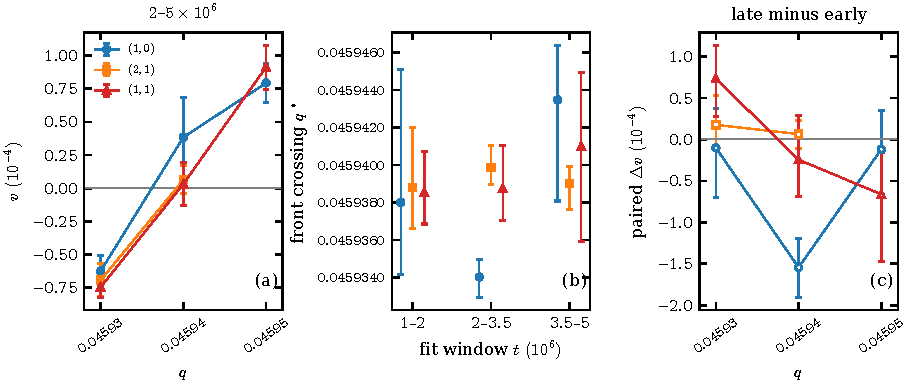
\includegraphics[width=\textwidth]{figs/fig_gpu_fronts5m}
\caption{Independent long-time front test at $p=\alpha=1/2$,
$L=8192$, with four new seeds per $(q,\mathrm{normal})$ and $T=5\times10^6$.
These cohorts are separate from the original $T=2\times10^6$ cohorts.
(a) Normal velocities fitted over $2$--$5\times10^6$, with one standard
error over runs. (b) Local bracketing crossings in successive windows
within the new cohorts, with conditional 95\% run-bootstrap intervals.
(c) Paired differences $v_{3.5\text{--}5\times10^6}-v_{2\text{--}3.5\times10^6}$;
each difference uses the same run in both windows, and bars are 95\%
run-bootstrap intervals. The profile threshold is 0.3. Only complete
predeclared four-seed groups with valid separated-front geometry throughout
both windows contribute. Threshold and interpolation choices remain
separate systematic uncertainties.}
\label{fig:gpu_fronts5m}
\end{figure*}

A further independent axial grid extends the same three probabilities to
$10^7$ steps, again with four new seeds per probability. All twelve runs
retain valid band geometry in both the $2$--$5\times10^6$ and
$5$--$10\times10^6$ windows at all three thresholds. At threshold 0.3,
the local crossing changes from 0.0459372 to 0.0459412; the paired shift
is $4.0\times10^{-6}$ with a conditional 95\% interval
$[2.4,5.6]\times10^{-6}$. The shift remains positive at thresholds 0.2
and 0.5, whose late crossings are 0.0459413 and 0.0459407. The threshold estimator retains residual time dependence in this
independent extension. Its precision is estimator-dependent, as shown
by the integrated-observable comparison below; it does not demonstrate
stationarity. At $q=0.04594$, all four interiors retain more than 90\%
of their reference activity throughout the final window.

For common normalizations below, we adopt the rounded operational reference
$q^*=0.04594$ and vary it over $[0.04592,0.04596]$. This
sensitivity range contains the extended-front point estimates and the
conditional bootstrap intervals reported above; alternative small-sample
intervals can extend beyond it. It is not a pooled confidence interval or a bound
on the limiting coexistence point. The measured time and orientation contrasts
remain part of the physical resolution of the study.

A complementary test places a large droplet of each phase in the other~\cite{wang2015}.
The signs on either side test opposing invasion; shrinkage of both finite
droplets could also be caused by ordinary curvature near a single isotropic zero. Figure~\ref{fig:drop2} shows, at
$p = 1/2$ and $L = 4096$, an active disk of radius 1000 in the dead state and a dead hole of the same
radius in the active state, at $q=0.0456842$, 0.0458221, 0.0460979,
and 0.0462358. At every sampled $q$ one of the two grows
while the other shrinks: above $\qs$ the active disk grows and the hole closes, below $\qs$ the
disk shrinks and the hole opens, with rates compared to a planar-front velocity corrected for
curvature, $\ds R/\ds t = \pm v - D/R$ (Sec.~\ref{M-sec:drops}). The radius estimator and its spatial trimming are specified in
Sec.~\ref{app:numerics}. We compare the corrected growth-law integration
and alternative radius estimators using the same trajectories.
The disk and hole exchange their signs of growth between $q=0.0458221$
and 0.0460979. The primary mean disk rates differ from the integrated
curvature prediction by at most $2.65\times10^{-4}$ sites per step.
For holes the difference is at most $3.60\times10^{-4}$, except at
$q=0.0456842$, where it is $5.78\times10^{-4}$ and the surrounding
metastable active phase also begins to decay. Replacing the trimmed,
rectified area by the full signed area changes the mean hole rate at
$q=0.0458221$ from $0.710\times10^{-3}$ to $0.873\times10^{-3}$,
without changing its sign. The complementary growth signs persist in
every individual run at all four sampled probabilities.

These coarse droplet measurements locate opposing invasion tendencies.
They do not determine whether an asymptotic interval of generic
coexistence lies between the closest points. Even with a single isotropic
front reversal, the curvature law makes both droplets of a finite radius
shrink whenever $|v|<D/R$. Consequently, observing both finite droplets
shrink would also require a radius sequence before it could distinguish
such an interval from ordinary curvature. Here the central droplet gap
is $2.758\times10^{-4}$, well above the observed front-crossing differences.


\begin{figure*}
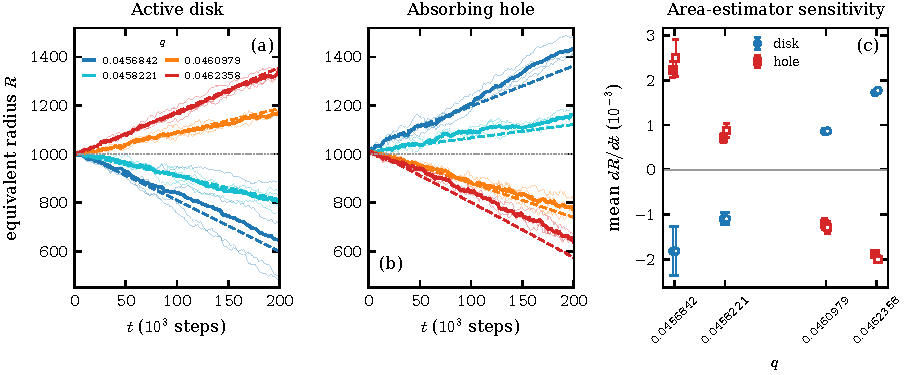
\includegraphics[width=\textwidth]{figs/fig_drop2}
\caption{Complementary droplets at $p=\alpha=1/2$, $L=4096$.
An active disk (a) and an absorbing hole (b) both start with radius 1000.
Thin solid curves show four individual runs per probability and thick
solid curves show their mean equivalent radius. The primary area estimator
uses the trimmed, nonnegative row chords defined in the numerical methods.
Dashed curves integrate $dR/dt=v-D/R$ for disks and $dR/dt=-v-D/R$ for
holes, with $D=0.20$, starting at the measured mean radius at
$t=2\times10^4$. The signed planar velocity $v$ is interpolated at the
actual $q$ from the corrected broad axial-front survey.
(c) Mean radius slopes fitted over $2\times10^4\le t\le2\times10^5$.
Filled markers use the primary trimmed and rectified area, open markers
the full signed area; their small horizontal offsets separate estimators
at the same $q$. Bars are one standard error across four runs.
All individual runs retain the displayed growth or shrinkage sign under
both area definitions.}
\label{fig:drop2}
\end{figure*}


We compare the profile-envelope velocities with slopes of three integrated
observables: twice the live-site fraction, the bond interface density, and
the fraction of sites with a disagreeing neighbor. Their fixed positive
normalizations set equivalent width units but do not move a velocity zero.
At $L=8192$ over $5$--$10\times10^6$ steps, the independent axial cohort
gives crossings 0.04594117, 0.04594063, 0.04594075, and 0.04594075,
respectively. The operational reversal therefore changes little across
these estimators. These observables share the same trajectories and are
not independent confirmations.

At $L=16384$ over $1$--$2\times10^6$ steps, the axial-minus-tilted
crossing difference changes from $4.66\times10^{-6}$ for the envelope
to $2.70\times10^{-6}$ for integrated bond activity. The envelope's
conditional bootstrap contrast excludes zero, while a delta-method
Welch--Satterthwaite sensitivity interval, with Bonferroni adjustment over
three direction pairs, is $[-0.13,9.45]\times10^{-6}$. The apparent angular
separation is thus sensitive to the estimator and small-sample uncertainty
construction. The axial change within the independent $5\times10^6$ cohort
persists across all four observables. For the $10^7$ cohort, the envelope
shift of $4.00\times10^{-6}$ has a delta-method interval
$[1.66,6.34]\times10^{-6}$, whereas the bond-activity shift of
$2.61\times10^{-6}$ has interval $[-0.64,5.85]\times10^{-6}$.
These comparisons support the stated finite-time crossing resolution;
they do not establish a stationary, orientation-independent limit.



\section{Bulk density, spatial structure, and finite-size lifetimes}
\label{sec:sbulk}

The extended campaign resolves finite bulk activity close to front
reversal on large systems and long observation windows (Fig.~\ref{fig:gpu_bulk}). At $q=0.04594$, all four $L=8192$
random-start runs remain active through $5\times10^6$ steps. Their
unconditional mean density over $2.5$--$5\times10^6$ is $0.28659$, with a
pointwise 95\% run-bootstrap interval $[0.28651,0.28667]$.
The difference between the second and first halves of this late window is
$7.2\times10^{-5}$, with interval $[-8.7\times10^{-5},1.6\times10^{-4}]$.
Thus no systematic late-window density decrease is resolved at this sampled
point; the spatial and front checks test its relation to coexistence separately.
Doubling the size to $L=16384$ gives a mean of 0.28661 at the same $q$
and time window. All twelve $L=16384$ runs at $q=0.04592$, 0.04594,
and 0.04596 remain active through $5\times10^6$ steps; none of the
three cohorts resolves a late-window density drift. The corresponding
means are 0.28498, 0.28661, and 0.28803. This comparison extends the
finite-density branch to substantially larger systems near front reversal.
At $q=0.04594$, the matched $2$--$5\times10^6$ window gives
$\chi_{8192}/\chi_{4096}=0.97$ with a pointwise 95\% run-bootstrap
interval $[0.84,1.08]$. The four independent runs at each size show no resolved
increase of this magnetic fluctuation scale upon doubling $L$.
The further doubling gives $\chi_{16384}/\chi_{8192}=0.95$ with interval
$[0.78,1.14]$ over the same window, again with no absorption in either
four-run cohort.

\begin{figure*}
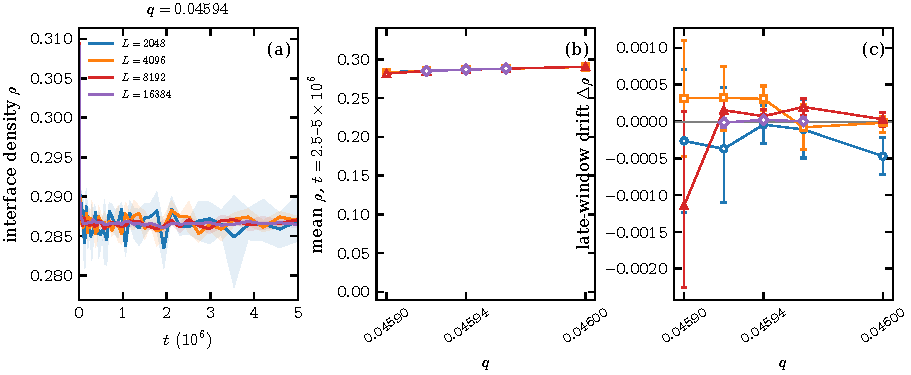
\includegraphics[width=\textwidth]{figs/fig_gpu_bulk}
\caption{Long, large-system bulk tests at $p=\alpha=1/2$, with four independent
random starts per $(L,q)$ and $T=5\times10^6$.
(a) Interface density at $q=0.04594$; bands are pointwise 95\% run-bootstrap
intervals. (b) Unconditional time-weighted density over
$2.5\times10^6\le t\le5\times10^6$ against the actual probability $q$.
(c) Difference between means over $3.75$--$5\times10^6$ and
$2.5$--$3.75\times10^6$; zero indicates no resolved drift between these
windows. Error bars in (b,c) are 95\% run-bootstrap intervals.
Every declared seed contributes; absorbed trajectories contribute their known
absorbing state for the rest of the observation window.}
\label{fig:gpu_bulk}
\end{figure*}

The final configurations provide a direct spatial check
(Fig.~\ref{fig:spatial_v2}). At $q=0.04594$, both $L=8192$ and 16384
give $C(128)\simeq0.0046$. For $L=16384$, $C(r)$ decreases from
0.427 at one lattice spacing to $5.7\times10^{-4}$ at $r=256$;
the pointwise intervals at $r=512$ and 1024 include zero. Signed
long-distance fluctuations are retained rather than clipped or fitted
to an assumed positive tail. The observed decay occurs on scales much
smaller than the box, complementing the density and magnetic-moment
comparisons. These are final-time measurements, not an extrapolation
of a correlation length to the transition.

\begin{figure*}
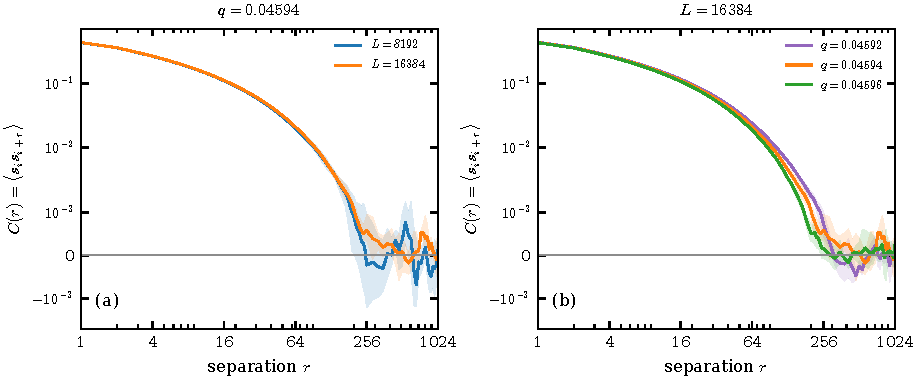
\includegraphics[width=\textwidth]{figs/fig_spatial_v2}
\caption{Direct spatial correlations at $p=\alpha=1/2$, measured in the
final configurations at $T=5\times10^6$, with four independent runs per
curve. The observable is the raw axis-averaged spin product in
Eq.~\eqref{M-eq:correlation}. (a) Size comparison at $q=0.04594$.
(b) Three probabilities at $L=16384$. Shading gives pointwise 95\%
run-bootstrap intervals; all declared configurations are included.
The vertical scale is logarithmic outside $|C|\le10^{-3}$ and linear
inside that interval, displaying both signs of the small long-distance
fluctuations. No functional form is fitted.}
\label{fig:spatial_v2}
\end{figure*}

Earlier bulk runs from random initial conditions (Fig.~\ref{fig:bulk}) give late-window
estimates of the active-phase interface density. At the points above $\qs$
shown in this survey, it settles within $10^3$--$10^4$ steps and then stays
constant to the end of the runs ($t = 2\times10^5$--$10^6$), independently of $L$ from 256 to 4096
within the run-to-run errors: $\rho = 0.3021$--$0.3023$ at $q = 0.046359$
and $0.3108$--$0.3113$ at $q=0.046818$
[Fig.~\ref{fig:bulk}(b)]. Even at $q = 0.0459$, the active phase
holds $\rho\simeq0.28$ for the full run ($10^6$ steps for $L\le 1024$, $3\times10^5$ and
$2\times10^5$ for $L = 2048$ and 4096) at every $L\ge 512$.
Such persistence can occur on the metastable side, so bulk persistence alone
does not locate the boundary. The finite-density branch persists to the
front-reversal region, supporting a discontinuity of order 0.28.
The magnetic second moment of the active phase,
$\chi_L = L^2\langle m^2\rangle$, grows toward the transition: its estimates are
$60$--$66$ at $q=0.05049$ and $305$--$463$ at $q=0.046359$ for $L=512$--4096.
At $q=0.0459$ they are of order $10^3$ for $L\ge1024$, with substantial
run-to-run uncertainty and no resolved growth with size. These data constrain magnetic fluctuations
at the sampled active points, rather than excluding an unsampled critical interval.
Measured directly from stored configurations at $q=0.046359$ ($L = 2048$,
$t\ge 10^5$), the two-point function of the local spin $s_i=2\sigma_i-1$
falls to $0.40$ at one lattice spacing. Local exponential fits give
$\xi = 15$--$18$ over $4\le r\le 40$ and $10\le r\le 60$; at $q=0.05049$,
$\xi = 7$--$9$.

On the sampled lower-$q$ side, the active phase exhibits metastable decay. At $q = 0.045441$ its density stays within 12\% of
the apparent active-branch plateau for $10^4$ steps and then collapses at an accelerating rate
[Fig.~\ref{fig:bulk}(a)]. The accelerating collapse and visible growth of absorbing
droplets [Fig.~\ref{M-fig:snap}(b)] support nucleation-driven decay.
Where droplets of opposite type meet, a layer of the active phase
remains between them (Sec.~\ref{M-sec:wall}), so $\rho$ does not drop to zero at once but to a slowly
coarsening network of wetted walls. The recorded half-density time $\tau$ grows steeply as
$q\to\qs$: $\tau = 3.4\times10^3$, $8.0\times10^3$, $1.6\times10^4$, $2.6\times10^4$, and
$7.0\times10^4$ at $q=0.04131$, 0.043605, 0.044523, 0.044982, and 0.045441.
It saturates at large $L$ [Fig.~\ref{fig:bulk}(c)]; at the closest of these points,
the means are $7.33$, $7.04$, $6.65$, and $6.70\times10^4$ for
$L=512$, 1024, 2048, and 4096. Many droplets nucleate independently, and the decay is a local
process (the multi-droplet regime of Ref.~\cite{rikvold1994}). Smaller systems ($L\le 128$) decay
sooner, because their size is only a few correlation lengths of the active phase, so that
the whole lattice can reach an absorbing state through one fluctuation.

\begin{figure*}
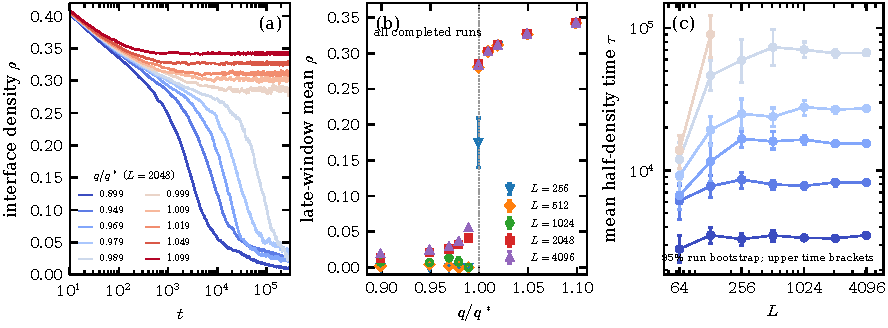
\includegraphics[width=\textwidth]{figs/fig_bulk05}
\caption{Bulk runs at $p = 1/2$ from random initial conditions ($\qs = 0.04594$). (a) Interface
density against time at $L = 2048$ for $q/\qs$ from 0.9 to 1.1 (one seed each).
(b) Time-weighted late-window density against $q/\qs$ for $L = 256$--4096,
using every completed run and all records over $t\ge T/2$ (2--16 runs per point).
Absorbed trajectories contribute zero after absorption; no activity filter is applied.
(c) Mean recorded half-density time below $\qs$ against $L$, shown only for
groups in which every trajectory crossed the threshold by the final time.
Times are first recorded crossings, including $10^3$ for five left-censored
$L=64$ runs; bars are 95\% run-bootstrap intervals, separate from output-cadence effects
(32 runs for $L\le
128$, 2--16 above; $T = 10^6$ for $L\le 1024$, $3\times10^5$ and $2\times10^5$ for $L = 2048$ and
4096).}
\label{fig:bulk}
\end{figure*}

The size dependence above $\qs$ is the opposite. Earlier $10^6$-step
cohorts at $q=0.046359$ had 32 of 32 consensus events at $L=64$, 25 of 32
at $L=128$, and none of 16 at $L=256$. We now test this stability signature
with independent, longer cohorts, keeping the two data sets separate.

A separate fixed ensemble extends the finite-size comparison at
$p=\alpha=1/2$, $q=0.046359$ to $T=10^7$ steps, with 32 independent
random starts at each of $L=64$, 128, 192, and 256
(Fig.~\ref{fig:lifetimes_v2}). The numbers reaching consensus are
32, 32, 6, and 0, respectively. The first recorded crossings of
$\rho<0.145$ are more frequent: 32, 32, 16, and 1.
Thus loss of half the reference activity and complete absorption are
separate observables. At $L=256$, the unconditional mean density over
$5\times10^6\le t\le10^7$ is 0.30230, with a 95\% run-bootstrap
interval $[0.30213,0.30246]$. With no consensus event among 32 $L=256$ runs,
the exact two-sided 95\% lower confidence limit for survival through
$10^7$ steps is 0.891. These observations extend the persistence window
and resolve strong size dependence; they do not determine an
asymptotic lifetime law.

The same contrast persists closer to coexistence. At $q=0.04605$, a
separate fixed ensemble follows 16 random starts at each of $L=192$,
256, and 384 to $3\times10^6$ steps. Consensus counts are 15, 6, and 0,
while recorded half-density events number 16, 6, and 1. The unconditional
mean densities over $1.5$--$3\times10^6$ are 0.060, 0.199, and 0.29235,
respectively. At $L=384$, the 95\% run-bootstrap density interval is
$[0.29100,0.29325]$,
and the exact two-sided 95\% lower confidence limit for survival through
the horizon is 0.794. Thus the size-dependent stability signature is
present at a second probability closer to the front-reversal region.

\begin{figure*}
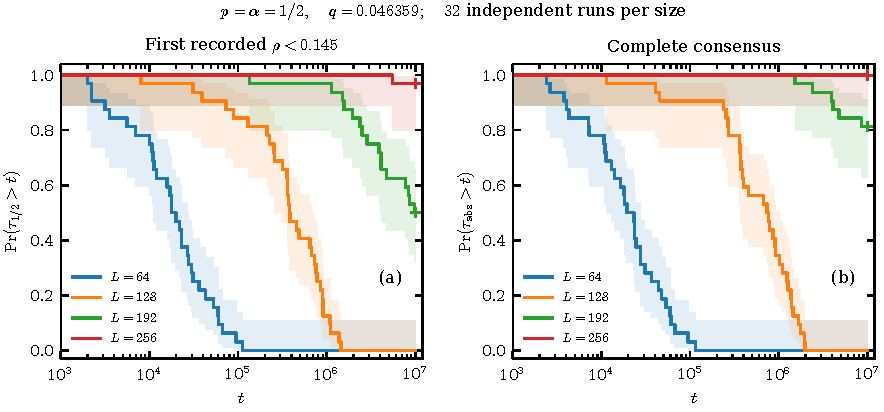
\includegraphics[width=\textwidth]{figs/fig_lifetimes_v2}
\caption{Long finite-size trajectories at $p=\alpha=1/2$, $q=0.046359$:
32 independent random starts per size, all followed until consensus or
$T=10^7$ steps. (a) Survival of the first recorded $\rho<0.145$ event,
searched at $t\ge10^3$ on the regular 1000-step and additional logarithmic
observation grid; recording-grid limitations are discussed in
Sec.~\ref{M-sec:methods}. (b) Survival to complete consensus.
Event counts for $L=64,128,192,256$ are $(32,32,16,1)$ in (a) and
$(32,32,6,0)$ in (b). Crosses denote right censoring. Shading gives
pointwise 95\% Kaplan--Meier bands (Greenwood log--log intervals away
from zero and one, with exact binomial edge bounds).}
\label{fig:lifetimes_v2}
\end{figure*}

In a multi-droplet description, the half-density time scales as
$\tau\propto(Iv^2)^{-1/3}$, where $I$ is the nucleation rate per unit area and
$v$ is the growth speed~\cite{rikvold1994}. The steep increase of $\tau$ on
approaching coexistence is consistent with slowing fronts and rarer nucleation.
Our finite interval of control parameters does not determine an asymptotic
nucleation law. In particular, a fit over these points cannot establish or
exclude the essential singularity expected from a classical nucleation barrier.


\section{Wall adsorption and local roughness}
\label{sec:swall}

A wall between all-alive and all-dead regions develops an active layer even when
the bulk active phase is metastable. Below the measured front reversal the
layer approaches a slowly varying thickness; above it the two edges move apart as active--absorbing
fronts. This geometry probes the competition among all three phases without
preparing an active region initially.

We measure the number $I=L_y\iota/2$ of interface sites per unit wall length and subtract
the $q=0$ value $I_0\simeq8.7$ to obtain the excess adsorption
$\Gamma=I-I_0$. Earlier measurements give an increase from about 10 at
$q=0.03672$ to about 109 at $q=0.0456705$. This increase is reproduced
across wall lengths $L_x=256$--4096 and transverse sizes $L_y=1024$--4096
(Fig.~\ref{fig:wall}). Runs last $10^6$--$3\times10^6$ steps.
For the late-window estimates we time-average each run over
$t\ge\max(3\times10^5,T/2)$ and then average independent runs.
Some walls wander far enough to consume one of the absorbing slabs. We terminate
their averaging windows before the live fraction leaves $[0.3,0.7]$, record
these truncations, and use the larger transverse boxes for the closest points.
The seven-point legacy fit below contains three truncated run windows and
omits one run with no usable window. Its two $L_y=4096$ points use the
available $L_y=1024$ baseline. The uncertainty of each shared $q=0$ baseline
is retained in the fit covariance; these legacy fits are conditional on the
stated geometry windows and baseline choices.

The increase of $\Gamma$ is robust, but a pure power law is sensitive to the
coexistence point and to corrections to scaling. With $q^*=0.04594$ and
$\delta=1-q/q^*$, fitting $\Gamma=A\delta^{-\psi}$ to the seven
$L_x=1024$, $L_y\ge2048$ points gives an effective $\psi=0.524$.
The fit is inadequate within the run-to-run errors: $\chi^2=74.7$ for five
degrees of freedom. The equally parameterized form
$\Gamma=A\delta^{-1/3}+B$ instead gives $A=20.28$, $B=-27.43$, and
$\chi^2=10.53$ for five degrees of freedom. Both fits minimize residuals in
adsorption units. Varying $q^*$ over $[0.04592,0.04596]$ moves the effective
pure-power slope from 0.506 to 0.541 and the offset-form $\chi^2$ from
3.74 to 27.03. An additive correction therefore changes the interpretation
of the apparent slope, while its fit quality remains reference dependent.
These legacy data do not establish an asymptotic exponent.

\begin{figure*}
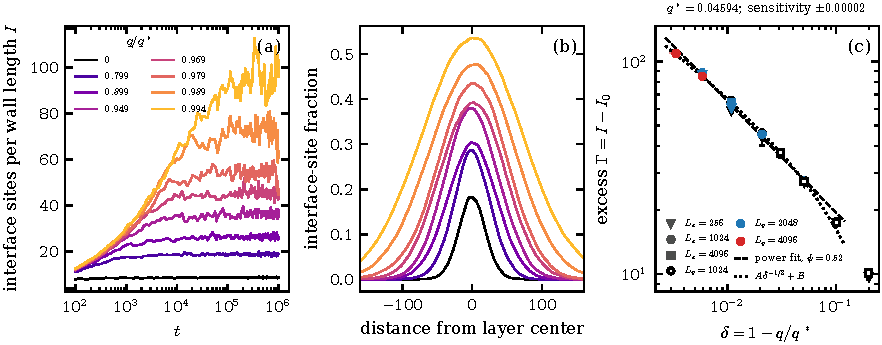
\includegraphics[width=\textwidth]{figs/fig_wall05}
\caption{Wetting at $p=1/2$, referenced to $q^*=0.04594$.
(a) Interface sites per unit wall length against time for $L_x=L_y=1024$
(four seeds per curve). (b) Interface-site fraction across the layer, centered
on its interface-weighted mean row before averaging late records.
(c) Excess adsorption for several box sizes (two to four seeds per point);
vertical bars show standard errors over runs including baseline uncertainty.
Horizontal bars on the fit points show the effect of varying $q^*$ by
$\pm0.00002$, a systematic sensitivity range. The dashed pure-power fit and
dotted $A\delta^{-1/3}+B$ fit use the same seven points with $L_x=1024$,
$L_y\ge2048$ and $\delta\le0.1$. The offset reduces the residuals, but neither fit determines the
asymptotic law.}
\label{fig:wall}
\end{figure*}

The extended test uses $L_y=8192$, wall lengths $L_x=4096$ and 16384,
and four independent $10^7$-step runs at each of three closer probabilities
(Fig.~\ref{M-fig:gpu_wetting}). Every ensemble is complete and retains the
full $5\times10^6$--$10^7$ averaging window, with a matched-size
$q=0$ baseline from two $2\times10^6$-step runs. All wall-separation
and global-density geometry checks pass. At $L_x=16384$, the excess
adsorptions are 133.27, 166.15, and 190.86 for $q=0.04584$, 0.04588,
and 0.04590. The corresponding $L_x=4096$ values are 134.80, 168.37,
and 199.90. At the closest probability, the larger system has about
4.5\% less adsorption; the run-bootstrap interval for this size difference
excludes zero. Its adsorption also declines by about 0.6\% between the
two halves of the late window, a small late-window change observed in all four runs.
These data extend the observed thickening while exposing finite-size
and finite-time corrections.

The new points test predictions from the earlier fits. At each fixed
front-derived reference, both candidate forms are fitted only to the
seven legacy points; their parameter uncertainty and shared-baseline
covariance are propagated to the predictions. Agreement at one new
probability does not imply a joint description of all three. The
extended measurements show discrepancies beyond their sampling errors
from the legacy extrapolations, together with the size and time effects
above. The analysis therefore does not assign an asymptotic wetting
exponent or treat either two-parameter extrapolation as a converged law.



The observed adsorption increase motivates a complete-wetting interpretation: near
coexistence an absorbing--absorbing interface separates into two
absorbing--active interfaces. Active boundary layers also occur between
defensive alliances~\cite{szabo2007}. In equilibrium, the interface between two
ordered phases can be wetted by the disordered phase at a first-order Potts
transition~\cite{selke1983,carlon1999}; fluctuating short-range interfaces in
two dimensions give the exponent $1/3$~\cite{lipowsky1983,fisher1984,carlon1999}.
Nonequilibrium wetting has also been studied with a bounded
Kardar--Parisi--Zhang interface~\cite{hinrichsen1997wet,munoz1998,delossantos2003}.
Here the layer is bounded by two fluctuating active--absorbing fronts.

The film edges show short-distance height-difference correlations close to
$\langle[h(x+r)-h(x)]^2\rangle\propto r$. Log--log fits over the recorded
separations $2\le r\le50$ give effective roughness exponents
$\zeta=0.468$, $0.499$, and $0.502$ for $L_x=256$, 1024, and 4096,
respectively. The local layer thickness has a broad distribution
(Fig.~\ref{fig:rough}). These finite-distance measurements motivate a
fluctuating-interface description, while the asymptotic exponent and
large-distance interaction remain unresolved.

\begin{figure*}
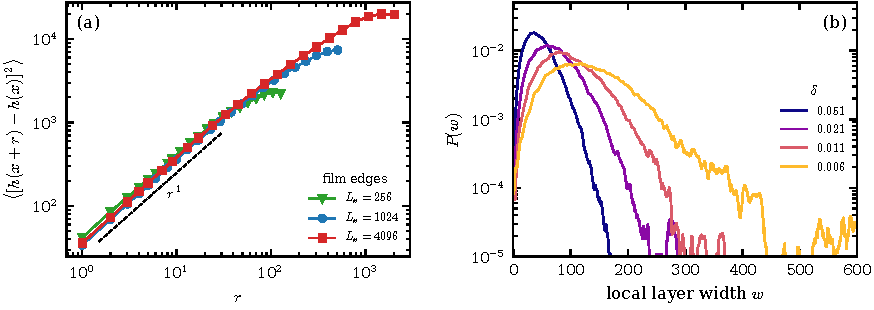
\includegraphics[width=\textwidth]{figs/fig_rough}
\caption{Edges of the wetting film at $p=\alpha=1/2$, from configurations
stored every $10^5$ steps for $t\ge10^5$, with $L_y=2048$.
(a) Height-difference correlation of both physical film edges at
$q=0.045441$, averaged equally over independent runs. The wall lengths
$L_x=256$, 1024, and 4096 have four, four, and two runs, respectively.
The dashed line shows $\propto r$, corresponding to $\zeta=1/2$.
(b) Local thickness distributions for $L_x=1024$ at $q=0.043605$,
0.044982, 0.045441, and 0.0456705. The legend gives
$\delta=1-q/q^*$ using $q^*=0.04594$. Curves show a five-bin moving
average of the run-averaged histograms.}
\label{fig:rough}
\end{figure*}

%=====================================================================================

\section{Parameter survey, long crossovers, and update timing}
\label{sec:sline}

\subsection{Phase diagram}
\label{sec:sphase}

Figure~\ref{M-fig:phase} shows the surveyed invasion boundary $\qs(p)$ from strip fronts at $\alpha = 1/2$,
together with the interface density of the active phase just above it. The line is nonmonotonic.
The directly simulated D\&N reference has $\qs(0)\approx0.0184$; the line
rises steeply at small positive $p$ (0.0207 already at $p = 0.01$)
to a maximum of $\approx 0.049$ near $p = 0.25$--$0.5$ and then approaches the voter
point approximately as $\qs\approx 0.25\,\alpha(1-p)$ over the sampled range
(Table~\ref{tab:line}). The initial rise is consistent with the voter
moves at $j = 4,5$, which D\&N forbids and which smooth interfaces.
The broad parameter survey finds sign-changing strip velocities and apparent
bulk plateaus $\rho_+ = 0.23$--$0.32$ at its stated observation times
[Fig.~\ref{M-fig:phase}(b)]. These finite-window densities do not determine the
limiting jump as $p\to1$. No tricritical point is resolved on this grid;
the longer-time assessment in Sec.~\ref{M-sec:voter} is essential near the endpoint.

\begin{table}
\caption{Broad finite-time survey at $\alpha=1/2$. Invasion thresholds
$\qs$ come from strip fronts (usually $L_x=2048$, $L_y=4096$, $T=10^5$,
2--4 seeds; $p=0$: five runs per probability across $L_x=2048,8192$;
$p\ge0.99$: note $b$), except for the refined $p=1/2$
estimate in Sec.~\ref{M-sec:fronts}. The bulk column gives the actual probability
$q_\rho$ and apparent plateau density $\rho_+$, using all selected runs at
$L\ge2048$ and time integration per run ($T\ge10^5$;
$p\ge0.98$: $T=10^6$--$1.5\times10^6$).
$c=\qs/[\alpha(1-p)]$. These densities are finite-window measurements.}
\label{tab:line}
\begin{ruledtabular}
\begin{tabular}{lllll}
$p$ & $\qs$ & $q_\rho$ & $\rho_+$ & $c$ \\
\hline
$0^{\,a}$ & 0.01837 & 0.0185 & 0.226 & -- \\
0.01 & 0.02070 & 0.021 & 0.245 & 0.042 \\
0.02 & 0.02280 & 0.02332 & 0.256 & 0.047 \\
0.05 & 0.02874 & 0.029 & 0.257 & 0.061 \\
0.1 & 0.03680 & 0.037904 & 0.288 & 0.082 \\
0.25 & 0.04932 & 0.05047 & 0.307 & 0.132 \\
0.5 & 0.04594 & 0.046359 & 0.302 & 0.184 \\
0.75 & 0.0276 & 0.0286 & 0.316 & 0.221 \\
0.9 & 0.01194 & 0.0122 & 0.290 & 0.239 \\
0.95 & 0.00619 & 0.0065 & 0.289 & 0.248 \\
0.98 & 0.00252 & 0.0025704 & 0.260 & 0.252 \\
0.99$^{\,b}$ & 0.00128 & 0.00128$^{b}$ & 0.241 & 0.256 \\
0.995$^{\,b}$ & 0.00064 & 0.00064$^{b}$ & 0.234 & 0.256 \\
\end{tabular}
\end{ruledtabular}
\begin{flushleft}\footnotesize
$^{a}$Direct $p=0$ reference, where the model has additional frozen configurations
(Supplemental Sec.~\ref{app:frozen}).\\
$^{b}$Runs of $1.2\times10^6$ ($p = 0.99$) and $1.6\times10^6$ steps ($p = 0.995$), four times the
crossover time $t_\times$ of Sec.~\ref{M-sec:voter}, four seeds, velocities fitted for $t\ge t_\times$
from the strip profile (Supplemental Sec.~\ref{app:numerics}); from runs of $10^5$ steps the
crossing at $p = 0.995$ is 0.00062 (Sec.~\ref{M-sec:voter}).
The bulk averages combine the nearby probabilities 0.00128 and 0.0012827 at
$p=0.99$, and 0.00064 and 0.0006417 at $p=0.995$; these are descriptive
survey values, not a limiting-density extrapolation. Their pooled standard
errors describe variation across these nearby parameters and horizons.
The new $2\times10^7$-step runs at $p=0.995$, $q=0.000640$ show
continuing decay (Sec.~\ref{M-sec:voter}); the tabulated threshold and density
there are historical finite-window estimates.
\end{flushleft}
\end{table}



\subsection{Near the voter point}
\label{sec:svoter}

As $p\to 1$ the transition approaches the voter point, where logarithmic corrections make every
diagnostic slow. A finite-window fit to one voter-model run at $L=4096$
gives $1/\rho\simeq0.184\ln t+2.13$ over $10^3\le t\le10^6$;
its slope depends on the fit start and is not an asymptotic amplitude.
A density that looks stationary over a finite window is therefore not enough.
We compare four complementary diagnostics at $p = 0.98$,
$0.99$, and $0.995$, with the noise strength measured by $\delta = q/\qs - 1$.

\textit{Bulk relaxation and front drift.} The earlier survey found apparent
plateaus $\rho\approx0.23$--$0.26$ over $10^6$--$1.5\times10^6$ steps at
$L=2048$ and 4096, including points very close to its estimated invasion
boundary. The sensitivity of that boundary to observation time already
signaled a long crossover. At $p=0.995$, a $10^5$-step strip estimate gives
$q\approx0.00062$, where the bulk subsequently decays; extending the strips
to $1.6\times10^6$ steps moves the crossing to approximately $0.000640$,
with a quoted spread of $5\times10^{-6}$ across the earlier estimates.
The analogous $1.2\times10^6$-step estimate at $p=0.99$ is about $0.00128$.
Table~\ref{tab:line} records this finite-time survey. Agreement between two
sizes over that horizon does not establish stationarity at longer times.
At $p=0.99$ the apparent plateau decreases on approaching the boundary:
$1/\rho$ changes from 3.60 at $q\approx1.19\,\qs$ to 4.11 near $\qs$.
These finite-window values alone distinguish neither a small limiting jump
nor logarithmically slow continuous vanishing.

The longer fixed ensembles at $p=0.995$ expose the limitation directly
(Fig.~\ref{fig:gpu_near}). At $L=4096$, the four-run mean density at
$q=0.000636$ falls from 0.201 over $10^6$--$2\times10^6$ steps to
0.027 over $5\times10^6$--$10^7$; all four runs reach consensus by
$10^7$. At $q=0.000640$, none reaches consensus by that time, but the
successive window means decrease from 0.228 to 0.216 to 0.207. At
$q=0.000644$ and 0.000648, the late means are 0.229 and 0.233 and no
late drift is resolved within the four-run uncertainty. These observations
separate collapse from persistence over a substantially longer horizon,
without identifying the limiting order parameter at the boundary.

Extending $L=8192$ runs to $2\times10^7$ steps makes the drift at
$q=0.000640$ clearer. The four-run mean falls from 0.189 over
$5\times10^6$--$10^7$ to 0.122 over $10^7$--$2\times10^7$,
with a 95\% run-bootstrap interval $[0.078,0.168]$ for the latter, and
one run reaches consensus. The difference between the second and first
halves of that window is $-0.055$, with interval $[-0.092,-0.027]$.
The earlier apparent plateau at this probability is therefore not a
stationary active-state measurement.
An independent midpoint ensemble at $q=0.000642$ retains activity in all
four runs, with late mean 0.2204 and interval $[0.2159,0.2231]$.
All four midpoint runs have a negative within-window change: $-0.0046$ with
interval $[-0.0077,-0.0015]$, about 2.1\% of its late mean. A paired $t_3$ reference interval is
$[-0.0109,+0.0016]$; the percentile interval has limited coverage accuracy
with four runs. We report the individual changes in Fig.~\ref{M-fig:gpu_near20m}
and do not assign a method-independent significance to the mean drift.
At $q=0.000644$ and 0.000648, all four $L=8192$ runs remain active
through $2\times10^7$, with late means 0.2265 and 0.2326 and no resolved
drift within $10^7$--$2\times10^7$. This separates late decay from
persistence on the sampled grid; bulk persistence alone still does not
locate an asymptotic coexistence boundary.
Figure~\ref{M-fig:gpu_near20m} shows the full largest-system time traces
and their paired late-window changes.

The strip experiment has a related limitation. At $q=0.000640$, activity
within the initial strip interior decays strongly and only one of four
runs retains valid separated-front geometry throughout
$5\times10^6\le t\le10^7$. An envelope fitted to the fragmented band
would mix front motion with internal decay. We therefore do not assign
a stationary front velocity to that ensemble. At higher $q$ the interior
persists, but expanding bands can instead encounter the finite box.
Both failures are visible in the width and interior-activity diagnostics.

\begin{figure*}
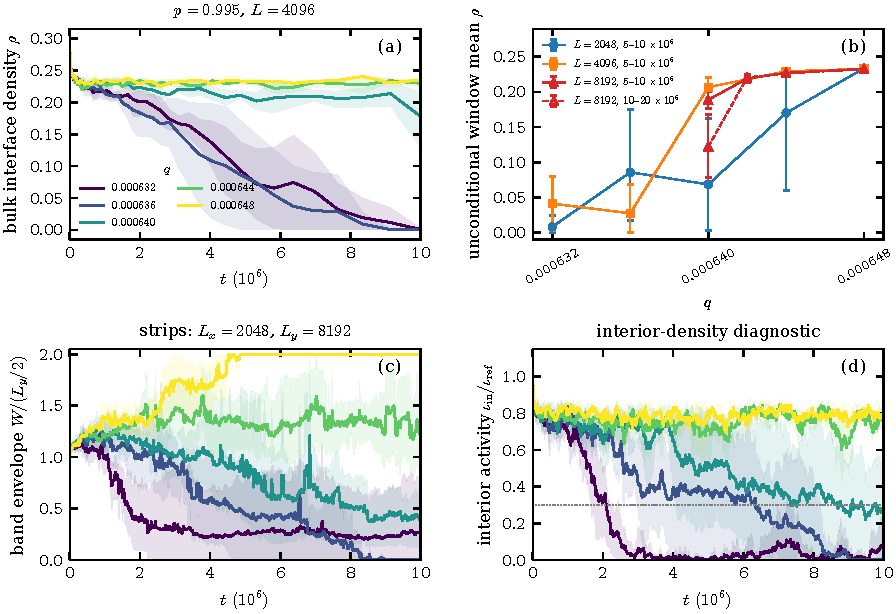
\includegraphics[width=\textwidth]{figs/fig_gpu_near}
\caption{Long-time tests near the voter point, $p=0.995$, $\alpha=1/2$;
four independent runs per parameter set. Colors in (a,c,d) denote the same $q$.
(a) Bulk density at $L=4096$ to $10^7$ steps.
(b) Unconditional time-weighted bulk means over the common
$5\times10^6\le t\le10^7$ window at three sizes, together with the later
$10^7$--$2\times10^7$ window at $L=8192$.
(c) Outer-envelope width of initially half-filled active strips,
$L_x=2048$, $L_y=8192$, normalized by the initial half-box width.
(d) Activity in the initial central interior region, relative to its
reference value at $t=10^3$. The dotted line is the profile threshold used
for the envelope. A changing interior density must be distinguished from
motion of a stationary front. Bands and bars are pointwise 95\%
run-bootstrap intervals. Absorbed trajectories are extended by their known
zero activity, and only complete predeclared seed ensembles are shown.}
\label{fig:gpu_near}
\end{figure*}



\textit{Size dependence of the magnetic fluctuations.} A split into an Ising
and a DP transition would leave an ordered active window. At the Ising point,
$\chi_L=L^2\langle m^2\rangle\sim L^{7/4}$, giving
$\chi_{4096}/\chi_{2048}=2^{7/4}\simeq3.36$.
Unfiltered, time-weighted run estimates show much weaker size dependence
at several sampled active points [Fig.~\ref{fig:voter}(a)]. For example,
at $p=0.98$, $q=0.0025704$, the ratio is $1.09$ with a pointwise
95\% run-bootstrap interval $[0.82,1.52]$.
Closer to the endpoint and threshold the uncertainty is larger:
at $p=0.99$, $q=0.0012827$, the ratio is $0.92$ with interval
$[0.34,4.20]$, and at $p=0.995$, $q=0.000651$, it is $1.95$
with interval $[1.07,3.46]$. These latter intervals include the Ising
size factor; restricting both sizes to the common window
$2\times10^5\le t\le5\times10^5$ leaves similarly large uncertainty.
No ordered active interval is resolved by the present grid,
but these measurements cannot exclude a narrower interval near the boundary.
The new $p=0.995$ ensembles at $q=0.000648$ give
$\chi_{4096}/\chi_{2048}=1.18$ with interval $[0.72,1.98]$ over the
common $5\times10^6$--$10^7$ window; all four runs at each size remain
active. This constrains fluctuations at that sampled active point.
The further doubling gives $\chi_{8192}/\chi_{4096}=0.91$ with interval
$[0.48,1.70]$ over the same window, also without absorption.
Closer to the boundary, absorption in the smaller systems contributes
$m^2=1$ and prevents interpreting an unconditioned size ratio as an
equilibrium critical-scaling test.

\textit{Suppression of small seeds.} A $2\times2$ block of live sites in the dead state
spreads, in the voter model, with survival probability $P_s(t)\simeq A\ln t/t$~\cite{bramson1980},
i.e., a local exponent $\delta_{\rm eff} = -\ds\ln P_s/\ds\ln t$ approaching 1 from below. GV criticality has voter-like asymptotic spreading, but this does not impose a finite-time bound on $\delta_{\rm eff}$ in a nonlinear model~\cite{castellano2012,azizi2020}; at a DP point $\delta_{\rm eff}\to0.451$. Figure~\ref{fig:voter}(b)
shows $t\,P_s(t)$, which grows as $\ln t$ for the voter model. At sampled
nonlinear-model points where the bulk remains active over the observation
window, this quantity instead decreases over substantial intervals.
The contrast is consistent with a nucleation barrier to invasion from
small seeds. At $p=0.99$, $q=0.0012954$, an independent predeclared
ensemble of $8\times10^6$ seeds leaves 19 survivors and no escapes at
$t=10^6$. Thus $P_s=2.375\times10^{-6}$, with an exact two-sided 95\%
binomial interval $[1.430,3.709]\times10^{-6}$. All sixteen fixed-size
shards of 500000 replicas completed with adaptive stopping disabled.
Between $t_1=63096$ and $t_2=251189$, the survival count falls from
793 to 97. The approximately factor-four-window estimate
$\delta_{\rm eff}=-\ln[P_s(t_2)/P_s(t_1)]/\ln(t_2/t_1)$ is 1.52,
with a pointwise 95\% conditional-binomial interval $[1.39,1.66]$.
The decay slope does not keep increasing: the last supported factor-four
window, $t=223872$--891251, gives 1.26 with interval $[0.99,1.59]$.
No terminal slope is quoted because 19 survivors fall below the
predeclared minimum count of 20. Overlapping windows are correlated
and are not fitted as independent exponent estimates. These observations
quantify intermediate-time seed suppression while leaving the asymptotic
survival probability and critical scaling unresolved.
At $p=0.995$, $q=0.0006324$, below the estimated threshold, none of
$3\times10^6$ seeds survives to $10^6$. Further above threshold the seeds
overshoot and then level off: at $p=0.99$, $q=0.0013335$, running to
$t=10^6$ on $L=8192$ gives 40 recorded survivors or escapes, compared with
88 at $10^5$. One of the terminal replicas has escaped, so the observed
late-retention ratio is bounded by $39/88$ and $40/88$, approximately
$0.44$--$0.45$, before sampling uncertainty; the voter asymptote gives
about 0.12. These higher-$q$ shards stopped at survivor targets, with
750839 replicas in total. Their curves are descriptive finite-time
evidence of slower late decay, and neither their stopping protocol nor
their observation horizon identifies a limiting survival probability.

\textit{Walls are wetted below the threshold.} A flat wall between the two absorbing phases
(protocol v) roughens like a voter interface at first, $W\propto t^{1/2}$, independent of $q$. After
a crossover time $t_\times$, $q$ takes over (Fig.~\ref{fig:voter}(c)). Below $\qs$ ($\delta =
-0.02$ at $p\le 0.98$, $-0.03$ at $0.99$, $-0.05$ at $0.995$) the wall turns into a slab of the
active phase with a long-lived finite width, $W(10^6)\approx 200$,
450, 670, and 820 for $p = 0.9$, 0.98, 0.99, 0.995, whose interior has an interface-site
fraction of 0.46--0.51, comparable to the earlier finite-window bulk estimates
near reversal (0.47--0.58); the pure voter wall
keeps widening. Above
$\qs$ the slab edges move outward at the strip-front velocities.
The crossover time increases from $\approx10^4$ at $p=0.9$ to
$\approx4\times10^5$ at $p=0.995$; the sampled-range fit
$t_\times\propto(1-p)^{-1.3}$ is an effective description, not an
asymptotic scaling law. This initial crossover marks the time at which
the perturbation becomes visible. The new longer runs show that it need
not mark final relaxation: the transition order remains unresolved at
$p=0.995$ and closer to the voter point.

These measurements follow the invasion boundary toward the voter point
and provide finite-time diagnostics of possible continuation of discontinuous behavior.
They do not establish that continuation at $p=0.995$, where threshold
uncertainty and relaxation times are largest. Accelerated seed extinction
supports a nucleation interpretation, rather than a universal finite-time
test excluding GV criticality. We distinguish these endpoint results from
the well-resolved coexistence at $p=1/2$ and from a claim about every fixed
$p<1$.

\begin{figure*}
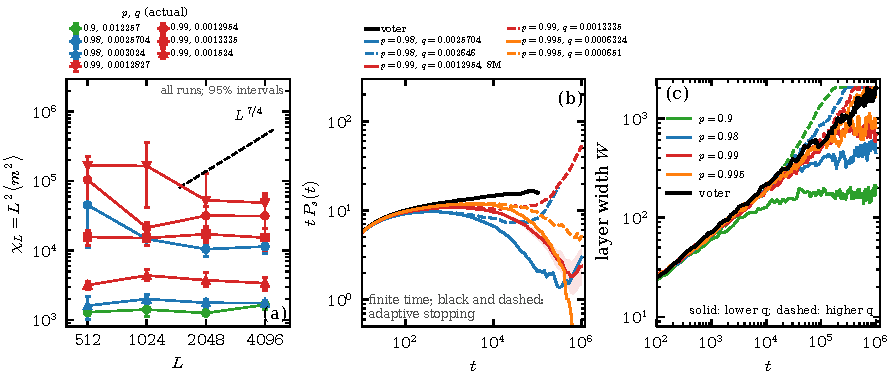
\includegraphics[width=\textwidth]{figs/fig_voter}
\caption{Near the voter point. (a) Unconditioned magnetic second moment
$\chi_L = L^2\langle m^2\rangle$ from random starts for $p=0.9$, 0.98,
and 0.99; the legend gives actual $q$. Each point averages 2--8 independent
runs after time integration over $t\ge2\times10^5$, with final times
$5\times10^5$ or $10^6$. Bars are pointwise 95\% run-bootstrap intervals.
No activity filter is applied: trajectories reaching consensus contribute
$m^2=1$ thereafter, which affects the small systems. The dashed line is
the Ising law $L^{7/4}$. (b) Survival of a $2\times2$ seed in
the dead state, $t\,P_s(t)$, which grows as $\ln t$ for the voter model (black, $L = 2048$), decays
when small seeds are strongly suppressed, and would grow linearly for a
positive limiting survival probability. The red solid curve at $p=0.99$,
$q=0.0012954$ uses the complete independent fixed-$N$ ensemble of
$8\times10^6$ replicas. Shading gives pointwise 95\% binomial intervals
(Clopper--Pearson for sparse counts, Wilson otherwise). Other nonlinear
solid curves retain the earlier $3\times10^6$-replica ensembles.
The black voter reference and higher-$q$ dashed curves use adaptive
survivor-target stopping and are shown descriptively.
The black reference stops at 300 retained replicas out of 1,905,766,
including 11 escapes at $t=10^5$; its plotted retained fraction is the upper
survival bound. Lattice size is
$L=8192$ for the nonlinear models; escapes are recorded separately.
(c) Width $W$ of the active
layer on a flat wall between the two absorbing phases, $L_x=1024$, $L_y=4096$,
two seeds. The pairs of lower (solid) and higher (dashed) probabilities are
$(0.011662,0.012495)$, $(0.0024696,0.002646)$,
$(0.0012446,0.0013335)$, and $(0.0006076,0.000651)$ for
$p=0.9$, 0.98, 0.99, and 0.995, respectively. Black: the voter model
($p=1$, $q=0$).}
\label{fig:voter}
\end{figure*}

\subsection{Synchronicity and asynchronous updating}
\label{sec:async}

The D\&N weight $\alpha$ sets the scale of $\qs$. Near the voter point the measured threshold is consistent with proportionality to $\alpha$: strip fronts at $\alpha = 1/4$, $1/2$, and 1 for $p = 0.98$ and 0.99 give
$\qs\propto\alpha^{\beta}$ with $\beta = 1.00\pm0.02$ and $c = \qs/[\alpha(1-p)] = 0.248$--$0.258$
(Table~\ref{tab:alpha}), consistent with the finite-time closure of
Sec.~\ref{M-sec:theory}. At the directly simulated $p=0$ reference, the
finite-density branch persists at the sampled $\alpha$ values between $1/8$
and 1, with no tricritical point resolved on that grid.

To test sensitivity to parallel updating, we make the dynamics lazy: each site
is updated with probability $r$ per step (the flip table is multiplied
by $r$), so $r\to 0$ is continuous time and $rt$ is the physical time. At $p = 0.98$ the front
velocity still changes sign. Nominal linear fits give
$\qs(r)/\qs(1) = 0.864\pm0.010$, $0.858\pm0.016$,
and $0.870\pm0.012$ for $r = 1/2$, $1/4$, and $1/8$.
These legacy fits use selected profile windows and extrapolate slightly
beyond their fitted probability range. Alternative documented fit ranges
shift the ratios by as much as 0.05, beyond the quoted sampling errors.
No monotonic change among the sampled $r\le1/2$ is resolved within that
systematic variation. At
$p = 0.99$, $r = 1/4$, fronts just above $\qs(r)$ retreat for $\sim 10^5$ physical time units
before advancing, and the late-time crossing, $0.85$--$0.88$, agrees with $p = 0.98$. At the
representative point $p=1/2$, corrected outer-envelope tracking of three
strips over physical times $2.5\times10^4$--$5\times10^4$ gives a
finite-window crossing $q^*(1/4)\simeq0.03963$, or roughly 0.86 of the
synchronous value. Earlier windows and profile thresholds produce shifts
of several $10^{-3}$ in this ratio, so greater asymptotic precision is
not assigned. The bulk active phase at $q=0.040392$ has a late-window mean
$\rho\simeq0.2105$ through physical time $10^5$, while at $q=0.039474$
it decays slowly. Supporting near-voter runs show bulk plateaus over a
factor 40 in time at roughly 10\% above the nominal crossing, early seed
decay with $\delta_{\rm eff}>1$, and active wall layers below the nominal
crossing while the lazy-voter wall keeps widening. The legacy seed curves
use adaptive stopping, and boundary escapes contaminate their late retained
counts, so no survival plateau is inferred from them.
These finite-$r$ checks show robustness to reduced update probabilities.
Establishing the strict continuous-time transition requires an extrapolation
in $r$.

\begin{table}
\caption{Synchronicity and asynchrony near the voter point. Top: $\qs\propto\alpha$ (strip
fronts, four seeds; errors are seed bootstrap, systematic $\approx\pm2\%$). Bottom: lazy updating
with probability $r$ per step at $p = 0.98$ and $1/2$; $c(r)$ from simulation and, near the voter
point, from the theory of Sec.~\ref{M-sec:theory}. The $p=0.98$ bottom entries
are nominal finite-window, profile-selected estimates; parentheses give
sampling errors, while probability-fit-range changes shift their ratios
by up to 0.05. The $p=1/2$ entry uses the corrected envelope over physical
times $2.5\times10^4$--$5\times10^4$ and is rounded to reflect window and
threshold sensitivity. Theory entries use fixed dual time $T=65536$
for synchronous walks and physical dual time $rT=65536$ for lazy walks;
their parentheses include walk-sampling uncertainty only.}
\label{tab:alpha}
\begin{ruledtabular}
\begin{tabular}{lllll}
$p$ & $\alpha$ & $\qs$ & $c$ (sim.) & $c$ (theory) \\
\hline
0.98 & 0.25 & 0.001274(9) & 0.255 & \\
0.98 & 0.5 & 0.002515(19) & 0.252 & \\
0.98 & 1 & 0.005074(30) & 0.254 & 0.255(2) \\
0.99 & 0.25 & 0.000621(18) & 0.248 & \\
0.99 & 0.5 & 0.001292(7) & 0.258 & \\
0.99 & 1 & 0.002553(9) & 0.255 & \\
\hline
$p$ & $r$ & $\qs(r)/\qs(1)$ & $c(r)$ (sim.) & $c(r)$ (theory) \\
\hline
0.98 & 1/2 & 0.864(10) & 0.218 & 0.221(3) \\
0.98 & 1/4 & 0.858(16) & 0.216 & 0.206(4) \\
0.98 & 1/8 & 0.870(12) & 0.219 & 0.200(4) \\
0.5 & 1/4 & $\approx0.86$ & 0.159 & -- \\
\end{tabular}
\end{ruledtabular}
\end{table}

%=====================================================================================

\section{Monotonicity and mean-field theory}
\label{sec:mf}

The model is attractive (monotone) when $w(j)$ is nondecreasing in $j$ and $w(j)+w(8-j)\le 1$,
because a site's probability of being alive after an update then increases with the set of live
sites. The second condition holds for $q\le(1-\alpha)(1-p)$.
The first requires both $(1-p)\alpha\le p/8$, from $j=3\to4$,
and $q\le(1-p)\alpha+p/8$, from $j=2\to3$.
Thus, at $\alpha=1/2$ and in the tested range
$q\le(1-p)/2$, the model is nonmonotone for $p<0.8$ and monotone
for $p\ge0.8$. These conditions do not cover the $\alpha=1$ checks.
None of our arguments uses monotonicity. Finite-time front and seed signatures
also occur in the monotone region; the strongest coexistence evidence below
is at the nonmonotone value $p=1/2$.
Monotone nonlinear voter models with two absorbing states and an
active phase in two dimensions are known, the threshold voter
models~\cite{liggett1994}; what is at issue here is the order of the transition, not the
existence of an active phase.

At the level of a pair approximation on the Bethe lattice with $z = 8$ (Supplemental Sec.~\ref{app:pa}),
the absorbing states are linearly stable for every $p<1$ and the disordered active state is
stable as well over the parameter range checked. The approximation is bistable
throughout that range and does not single
out a transition point: in a spatial system the phase is selected by which phase invades the
other. Mean-field bistability is precisely the situation in which washout is expected in two
dimensions~\cite{castellano2009}. Whether the two-dimensional transition is discontinuous is
therefore a question about fronts and fluctuations, and it is the question the simulations
address.

\section{Frozen configurations at $p = 0$}
\label{app:frozen}

At $p = 0$ the flip table is $w(j) = \alpha R(j) + q\,\delta_{j,2}$, so every configuration in
which all sites have $j\in\{0,1,4,5\}$ is frozen. A local construction proves
that their number grows exponentially with area. Start from a checkerboard
on a torus whose lengths are divisible by four. Independently choose whether
to complement each $2\times2$ block with lower-left corner $(4a,4b)$.
For one complemented block, its four sites and the four exterior diagonal
corners have $j=5$; the other sites in its surrounding $4\times4$ square
retain $j=4$. The affected neighborhoods of different blocks are disjoint,
so every choice is frozen. Hence, with $N=L_xL_y$,
\begin{equation}
 \mathcal N_{\rm frozen}\ge 2^{N/16},\qquad
 \frac{\ln\mathcal N_{\rm frozen}}{N}\ge\frac{\ln2}{16}.
 \label{eq:frozenbound}
\end{equation}
This bound holds for every admissible $q$ at $p=0$.

Transfer-matrix counts on periodic strips of fixed widths $W=7$ and $8$
give a larger strip entropy, $\mathcal N_W\sim e^{s_WN}$ with
$s_W\approx0.32$ per site, against $\ln2\simeq0.69$ for all configurations.
These two strip widths do not determine the two-dimensional entropy density.
As a check,
on the $3\times3$ torus, where every site neighbors every other, the count is
$254 = 1 + \binom94 + \binom95 + 1$. The simplest examples are the two checkerboards and the
diagonal stripes of width two, in which every site has $j = 4$.

These exceptional configurations did not attract the tested random starts at $q>0$. Random initial conditions at $L = 256$
run to $t = 10^6$ at $q = 0.005$--$0.018$ (all below $\qs$) end in one of the two uniform states.
In the active phase ($q = 0.03$--$1$) the frequency of locally checkerboard or stripe-like
$3\times3$ blocks stays at the level expected by chance. A prepared half-lattice of either pattern
next to an active or a dead half is eroded completely within $10^4$ steps at every $q$ tested,
including $q = 0$, and a single flipped site destroys a perfect $256\times256$ pattern within
$\approx 10^3$ steps (in 11 of 12 runs). Only at $q = 0$, where $j = 2$ sites are also frozen, does
the dynamics stop with a small density ($\approx 1\%$) of frozen debris.

Removing the frozen configurations directly by a flip probability $\epsilon$ at
$j\in\{1,4,5\}$ preserves the linear reversal of the front velocity: at $\epsilon = 0.003$ the
velocity is $-0.0041$, $-0.0002$, $+0.0024$, $+0.0053$ at $q/\qs(0) = 0.88$, 0.92, 0.96, 1.00, so
$\qs(\epsilon)\approx 0.92\,\qs(0)$, and at $\epsilon = 0.01$, $\qs\approx 0.8\,\qs(0)$, with
an interior interface fraction 0.44--0.6 behind the front. These checks retain
front reversal and an active interior after removing the extra frozen states.
They suggest a smooth small-$\epsilon$ continuation over the measured range;
they do not establish the infinite-time $p\to0^+$ limit of the voter-admixed family.

\section{Pair approximation}
\label{app:pa}

We closed the dynamics at the level of nearest-neighbor pairs on a Bethe lattice with $z = 8$:
given a site's state, its neighbors are independent and disagree with it with probability
$\theta_s = \rho/(2x_s)$, where $\rho$ is the fraction of disagreeing bonds and $x_s$ the fraction
of sites in state $s$. Both the continuous-time version and the synchronous map were analyzed.
In the voter limit the continuous-time closure conserves $m$ and gives $\rho^*=(z-2)(1-m^2)/[2(z-1)]$. The synchronous map differs: at $m=0$ its active fixed point is $\rho^*=1/2$. For every
$p<1$ a dilute minority in an absorbing state decays at rate
$(1-p)\alpha P_R(\theta) + qP_2(\theta)$, where $\theta$ is the conditional
disagreement probability around a minority site,
$P_j(\theta)=\binom{8}{j}\theta^j(1-\theta)^{8-j}$, and
$P_R=P_3+P_6+P_7+P_8$. Thus the absorbing states are linearly stable in the
parameter range studied, and the
symmetric active fixed point ($\rho^*\approx 0.43$--$0.50$) is stable over the
parameter grid checked. The approximation is bistable over that grid and
does not select a coexistence point; a
front criterion based on it gets $\qs\propto(1-p)$ near the voter point but with an amplitude off
by a factor of two, and fails qualitatively for $p\lesssim 0.5$. This motivates the finite-time closure examined in Sec.~\ref{M-sec:theory}.

\section{A second rule: noise on the forbidden flips of D\&N}
\label{app:eta}

To check that the discontinuity does not depend on the voter admixture, we studied the rule
\begin{equation}
w(j) = \alpha R(j) + \eta\,[\,j\in\{1,2,4,5\}\,],
\label{eq:eta}
\end{equation}
in which every flip that D\&N forbids, except at $j = 0$, happens with a small probability $\eta$.
For $0<\alpha,\eta\le1$, the lemma of Sec.~\ref{M-sec:lemma} gives exactly
two absorbing states. At $\alpha = 1/2$, strip
fronts ($L_x = 2048$, $L_y = 4096$, $T = 10^5$, three seeds) retreat at $v = -0.0022\pm0.0010$ for
$\eta = 0.01275$ and advance at $v = +0.0020\pm0.0001$ and $+0.0054\pm0.0001$ for $\eta = 0.013125$
and $0.01375$, so $\eta^*\approx 0.0130$ (linear interpolation: $0.01295$). Bulk runs at $L = 1024$ and 2048 (two seeds each,
$T = 2\times10^5$) have last-half interface densities
$\rho\simeq0.25$ at $\eta = 0.013125$ ($\approx
1.01\,\eta^*$) and $\rho\simeq0.276$ at $0.01375$, at both sizes. Below $\eta^*$ the prepared active phase decays: at $\eta = 0.01275$ it decays slowly (from $\rho = 0.236$ at $t = 10^4$ to $0.17$ at
$2\times10^5$), and at $\eta = 0.0125$, $0.01225$, $0.011875$, and $0.01125$ its half-life is
$(5.3$--$6.4)\times10^4$, $(2.6$--$3.2)\times10^4$, $(1.3$--$1.6)\times10^4$, and $(0.8$--$0.9)
\times10^4$, similar at the two sampled sizes. Here the half-life is the first
recorded crossing below half the density at $t=10^3$, rather than consensus.
Together these finite-window front and bulk checks support a discontinuity
with an active-side density of order 0.25 in this second rule
(Fig.~\ref{fig:eta}).

\begin{figure}
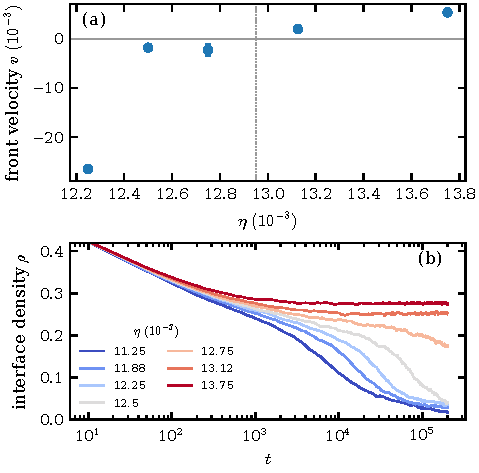
\includegraphics[width=\columnwidth]{figs/fig_eta}
\caption{The rule of Eq.~\eqref{eq:eta} at $\alpha = 1/2$. (a) Strip-front velocity against $\eta$
(three runs per $\eta$; plotted means retain fits with at least 20 records,
including only two runs at $\eta=0.01225$). The strongly negative
$\eta=0.01225$ estimate uses a short window before the strip interior orders;
it is not a late planar-front velocity. The dotted line is
$\eta^*=0.01295$. (b) Example bulk trajectories (seed 1) at $L=2048$.}
\label{fig:eta}
\end{figure}


\section{The five-cell rule of Molofsky \emph{et al.}}
\label{app:molofsky}

\textit{Rule and closure.} The synchronous square-lattice rule of
Ref.~\cite{molofsky1999} assigns a site the state 1 with probability $p_n$,
where $n$ counts state-1 sites in its von Neumann neighborhood including
itself. Here $p_0=0$, $p_5=1$, $p_3=1-p_2$, and $p_4=1-p_1$.
Equivalently, a site with $j$ disagreeing neighbors flips with probability
$w(j)=p_j$. For $0<p_1,p_2<1$, every nonuniform configuration permits a
flip, giving exactly two absorbing configurations. The voter point is
$(p_1,p_2)=(1/5,2/5)$, where a site copies one of these five cells uniformly.

Write $w(j)=j/5+g(j)$, with
$g=(0,\delta_1,\delta_2,-\delta_2,-\delta_1)$ and
$(\delta_1,\delta_2)=(p_1-1/5,p_2-2/5)$. The voter dual consists of five
coalescing walks, each staying or moving to any nearest neighbor with
probability $1/5$. Averaging over $10^7$ recorded walk realizations at each
cutoff gives the finite-time reaction function
\begin{equation}
 \begin{gathered}
 f_T(u)=u(1-u)(1-2u)[a+c\,u(1-u)],
 \\
 c=P_5(T)(10\delta_2-5\delta_1),
 \end{gathered}
 \label{eq:fmol}
\end{equation}
where $a=\delta_1a_1(T)+\delta_2a_2(T)$ and $P_5$ is the probability that
all five lineages remain distinct. The coefficients $a_1,a_2$ include all
lineage patterns. Within the constant-diffusion scalar closure,
$f_T'(0)=a$, $f_T'(1/2)=-(a+c/4)/2$, and
$\int_0^{1/2}f_T(u)\,\ds u=(6a+c)/192$.
For $c>0$, the sector $-c/4<a<0$ is bistable, and its stationary front lies
at $a=-c/6$.

Table~\ref{tab:molofsky} and Fig.~\ref{fig:molofsky}(a,b) show the narrowing
of this sector with cutoff. The conditional probability
$\Pr(K\ge5\mid K\ge3)$, where $K$ is the surviving lineage count, is
smaller for the five-cell neighborhood than for the nine-cell Moore
neighborhood by factors 10.5, 17.2, 28.6, and 45.3 at
$T=16,64,1024,65536$. This comparison concerns the weight of higher-degree
contributions among patterns that can contribute to the drift. Ref.~\cite{molofsky1999}
found that isolated seeds can nucleate expanding patches in the spatial
model and did not observe the multiple-outcome regime of its mean-field map.

\begin{table}
\caption{Finite-time closure for the five-cell rule. Angles in degrees
are measured from the $+\delta_1$ axis. The columns give the absorbing-state
stability threshold, stationary-front condition, active-state stability
threshold, and sector width of the deterministic closure. The $10^7$
walk realizations give bootstrap standard errors below $0.05^\circ$ for
each angle.}
\label{tab:molofsky}
\begin{ruledtabular}
\begin{tabular}{rrrrrr}
$T$ & $P_5/P_{\ge3}$ & $\theta_a$ & $\theta_f$ & $\theta_{1/2}$ & width\\
\hline
16 & 0.0664 & 104.34 & 107.28 & 108.77 & 4.43\\
64 & 0.0253 & 105.32 & 106.60 & 107.25 & 1.92\\
256 & 0.011 & 105.73 & 106.32 & 106.62 & 0.90\\
1024 & 0.00520 & 105.93 & 106.23 & 106.38 & 0.45\\
4096 & 0.0027 & 106.03 & 106.19 & 106.27 & 0.24\\
65536 & 0.000784 & 106.09 & 106.14 & 106.17 & 0.07\\
\end{tabular}
\end{ruledtabular}
\end{table}

\textit{Expansion and interior decay.} We simulated the cuts $p_2=0.45$
and $0.50$ using random active strips, bulk random starts, $2\times2$ seeds,
and active disks. The fine strip scan uses $L_x=2048$, $L_y=4096$,
$T=10^5$, and four runs per point, supplemented by two runs per point at
$L_x=4096$. Profiles are smoothed over 32 rows. We measure half the slope
of the width using either a fixed half-reference threshold, half the
contemporaneous central activity, or the integrated activity divided by
the contemporaneous central activity. Fits retain records with fixed-threshold
width between $0.1L_y$ and $0.9L_y$ and central activity above 60\% of its
reference at $t=10^3$.

The mean normalized central activity decreases by at most 0.03 between
$t=3\times10^4$ and $10^5$ at three $L_x=2048$ points on each cut.
Their adaptive-width slopes are all positive. Equal-weight linear fits to
these three group means, using records from $t=2000$, extrapolate to zero
at $p_1^{\rm ext}=0.185345$ and 0.170569. Changing the fit start to
$t=30000$ and using the three width estimators gives the ranges in
Table~\ref{tab:molsim}. These are finite-window estimates of expansion onset.
The fitted adaptive branch has no negative-velocity point with a comparably
persistent interior to bracket its zero.

At $(p_2,p_1)=(0.45,0.18535)$, the normalized interior activity falls
from 0.781 to 0.705 between $3\times10^4$ and $10^5$. Its adaptive slope
changes from $+0.000216$ to $-0.000829$ when the fit start changes from
2000 to 30000. At $(0.50,0.17057)$ the corresponding activity falls from
0.818 to 0.754, and the slopes are $+0.000036$ and $-0.000057$.
These contracting profiles combine edge motion and interior decay.
The extrapolated onset directions are approximately $106.3^\circ$--$106.4^\circ$,
close to the large-cutoff closure and the chord from the voter point to
$(0.024,1)$ in Ref.~\cite{molofsky1999}. Their precision is limited by
relaxation and estimator choice.

\begin{table}
\caption{Five-cell simulations. The zero is extrapolated from the three
positive adaptive-width slopes satisfying the stated interior-drift criterion.
The range varies the width estimator and fit start and gives a sensitivity
assessment. Each run reaches $10^5$ steps. The final rows give bulk interface
densities at the stated actual probabilities and observation horizons.}
\label{tab:molsim}
\begin{ruledtabular}
\begin{tabular}{lll}
 & $p_2=0.45$ & $p_2=0.50$\\
\hline
$p_1^{\rm ext}$ & 0.185345 & 0.170569\\
Range lower bound & 0.185345 & 0.170569\\
Range upper bound & 0.185397 & 0.170607\\
Smallest fitted $p_1$ & 0.185400 & 0.170620\\
$p_1$ of bulk sample & 0.185400 & 0.170620\\
$L$ & 2048 & 2048\\
Bulk horizon & $1.2\times10^6$ & $3\times10^5$\\
Late $\rho$ & $0.188(1)$ & $\approx0.20$\\
\end{tabular}
\end{ruledtabular}
\end{table}

\begin{figure*}
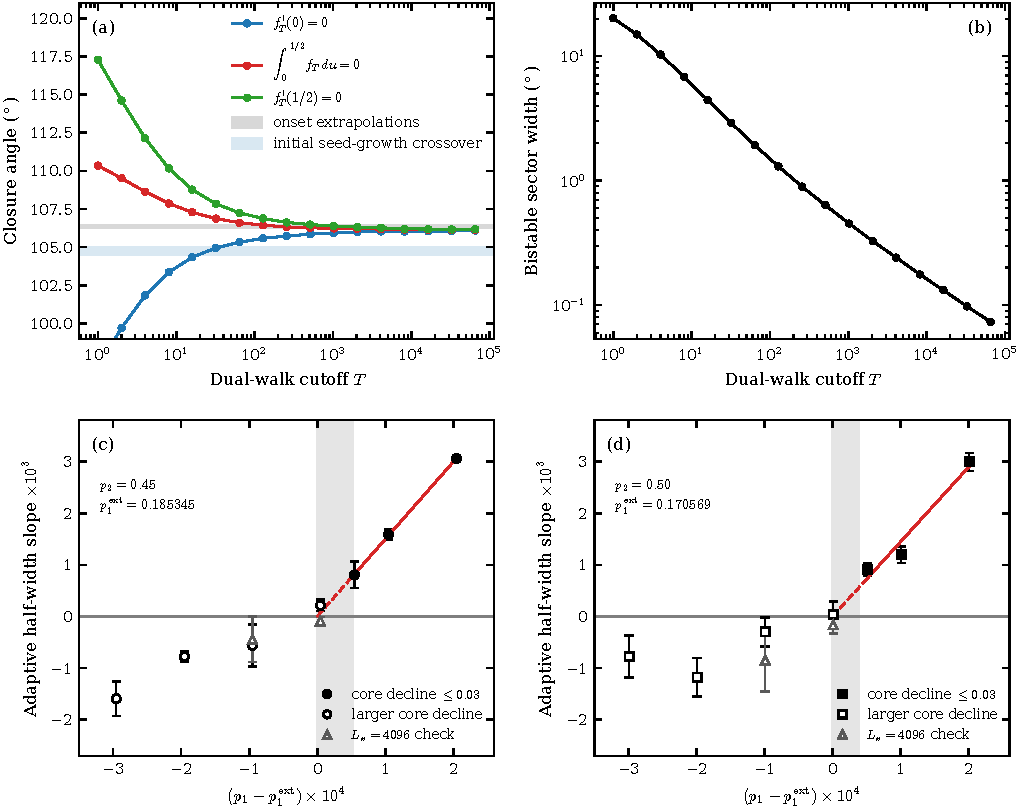
\includegraphics[width=\textwidth]{figs/fig_molofsky}
\caption{Five-cell closure and finite-time strip dynamics.
(a) Closure threshold angles versus dual-walk cutoff. Gray shading spans the
extrapolated onset angles from the two cuts, three width estimators, and two
fit windows. Blue shading marks the approximate initial seed-growth crossover
reported in the sampled ensembles. (b) Angular width of the closure's bistable
sector. (c,d) Half-slopes of the adaptive strip width from records with
$t\ge2000$ on the two cuts, with one standard error over runs. Filled points
have an ensemble-mean normalized interior decline of at most 0.03 between
$3\times10^4$ and $10^5$; open points show stronger interior decay.
Triangles are the two-run $L_x=4096$ checks; circles and squares are four-run
$L_x=2048$ groups. Solid segments fit the three filled $L_x=2048$ points,
and dashed segments extrapolate to zero. Gray bands give the corresponding
estimator/window ranges. The horizontal origin is the displayed early-window
adaptive extrapolation $p_1^{\rm ext}$.}
\label{fig:molofsky}
\end{figure*}

\textit{Seeds, bulk relaxation, and absorption.} The mean population of
$2\times2$ seeds initially decreases up to approximately $p_1=0.187$--0.188
on the first cut and 0.173--0.174 on the second. At $(p_2,p_1)=(0.45,0.186)$,
93 of 20000 seeds survive to $10^4$ steps. Active disks have finite-time
half-survival radii $R_{1/2}(2\times10^4)$ with products
$R_{1/2}v=0.1595$--0.1846 in four sampled cases, comparable with the voter
diffusion coefficient $1/5$. A fifth case gives $R_{1/2}>28$.
All recorded escape counts are zero. The ensembles stop at 100 survivors
or 400 replicas for disks and 300 survivors or 20000 replicas for small
seeds. Their endpoint proportions describe these adaptive samples.

At $p_2=0.45$, bulk runs at $p_1=0.18540$ have late mean
$\rho=0.188(1)$ for $L=2048$ through $1.2\times10^6$ and $0.190(1)$ for
$L=4096$ through $6\times10^5$. Nearby $p_1=0.18538$ and 0.18539 runs show
continuing drift or broad run-to-run variation. Logarithmic vanishing,
a small power, and a finite jump can describe the sampled density curve
when its boundary location is varied. This leaves the transition order open.

At the earlier reference values $p_1=0.18535$ and 0.17057, the all-run
restricted mean absorption times $\langle\min(T_{\rm abs},10^6)\rangle$
are $2.413\times10^5$ and $2.321\times10^5$ at $L=256$, increasing to
$5.942\times10^5$ and $8.539\times10^5$ at $L=512$. Each ensemble contains
four runs. All four absorb at $L=256$, whereas three absorb at $L=512$;
the remaining run contributes its full observation horizon. The density
relaxes through coarsening, and these runs resolve no persistent active
slab retreating as a coherent phase.

The observations place expansion onset, early seed suppression, and loss
of an apparent bulk plateau on different finite-time scales. These
observables offer tests of the closure, whose spinodal thresholds refer
to the deterministic reaction equation. The simulations resolve neither
those spinodals nor a metastable active branch for the five-cell rule.
A closure calibrated only to expansion onset therefore does not explain
the stronger coexistence signatures of the D\&N model.

\bibliography{refs}
\end{document}
